\documentclass[10pt,aspectratio=169]{beamer}

\usepackage[utf8x]{inputenc}
\usepackage[T1]{fontenc}
\usepackage{lmodern}

\usepackage{amsmath,amssymb,mathtools}
\usepackage{bm}
\usepackage{cancel}
\usepackage{empheq}
\usepackage{graphicx}
\usepackage{array,booktabs,tabularx,tabulary,multirow}
\usepackage{tikz}
\usepackage{hyperref}
\usepackage{feynmp}

\newcolumntype{V}{>{\centering\arraybackslash} m{.2\linewidth} }

\usetikzlibrary{arrows,matrix,shapes,positioning}
\usetikzlibrary{calc}
\usetikzlibrary{shadows.blur}

\newcommand*\widefbox[1]{\fbox{\hspace{0.5em}#1\hspace{0.5em}}}
\newcommand{\DRbar}{{\overline{\textrm{DR}}}}
\newcommand{\SUSYv}{{\cancel{SUSY}}}

\DeclareMathOperator{\Tr}{Tr}
\DeclareMathOperator{\STr}{STr}

\DeclareGraphicsRule{*}{mps}{*}{}
\graphicspath{{./figures/}}

\title{Minimal Supersymmetry and Beyond}

\author{D.~Harries\\
  {\scriptsize
  (IPNP, Charles University in Prague)}
  }

\titlegraphic{
  \begin{center}
    \hspace*{\fill}
    
\includegraphics[scale=0.3]{uk_logo}
    \hspace*{\fill}
  \end{center}
}

\date[\'{U}TF, Charles University in Prague]{March 27, 2018}

\usetheme{CambridgeUS}

\setbeamertemplate{headline}[default]{}
\setbeamertemplate{footline}[page number]{}
\setbeamertemplate{navigation symbols}{}

\begin{document}

\begin{frame}[plain]
  \titlepage
\end{frame}

\begin{frame}
  \frametitle{Outline}
  \tableofcontents
\end{frame}

% general aspects of SUSY
\section{General Features}

% very general mention of some empirical reasons for BSM
% physics before specialising to the theoretical motivations
% for studying SUSY as a feature of BSM models
\begin{frame}
  \frametitle{The Case for BSM Physics}
  \begin{columns}[t]
    \begin{column}{0.3\textwidth}
      \vspace*{-15pt}
      \begin{figure}
        \centering
        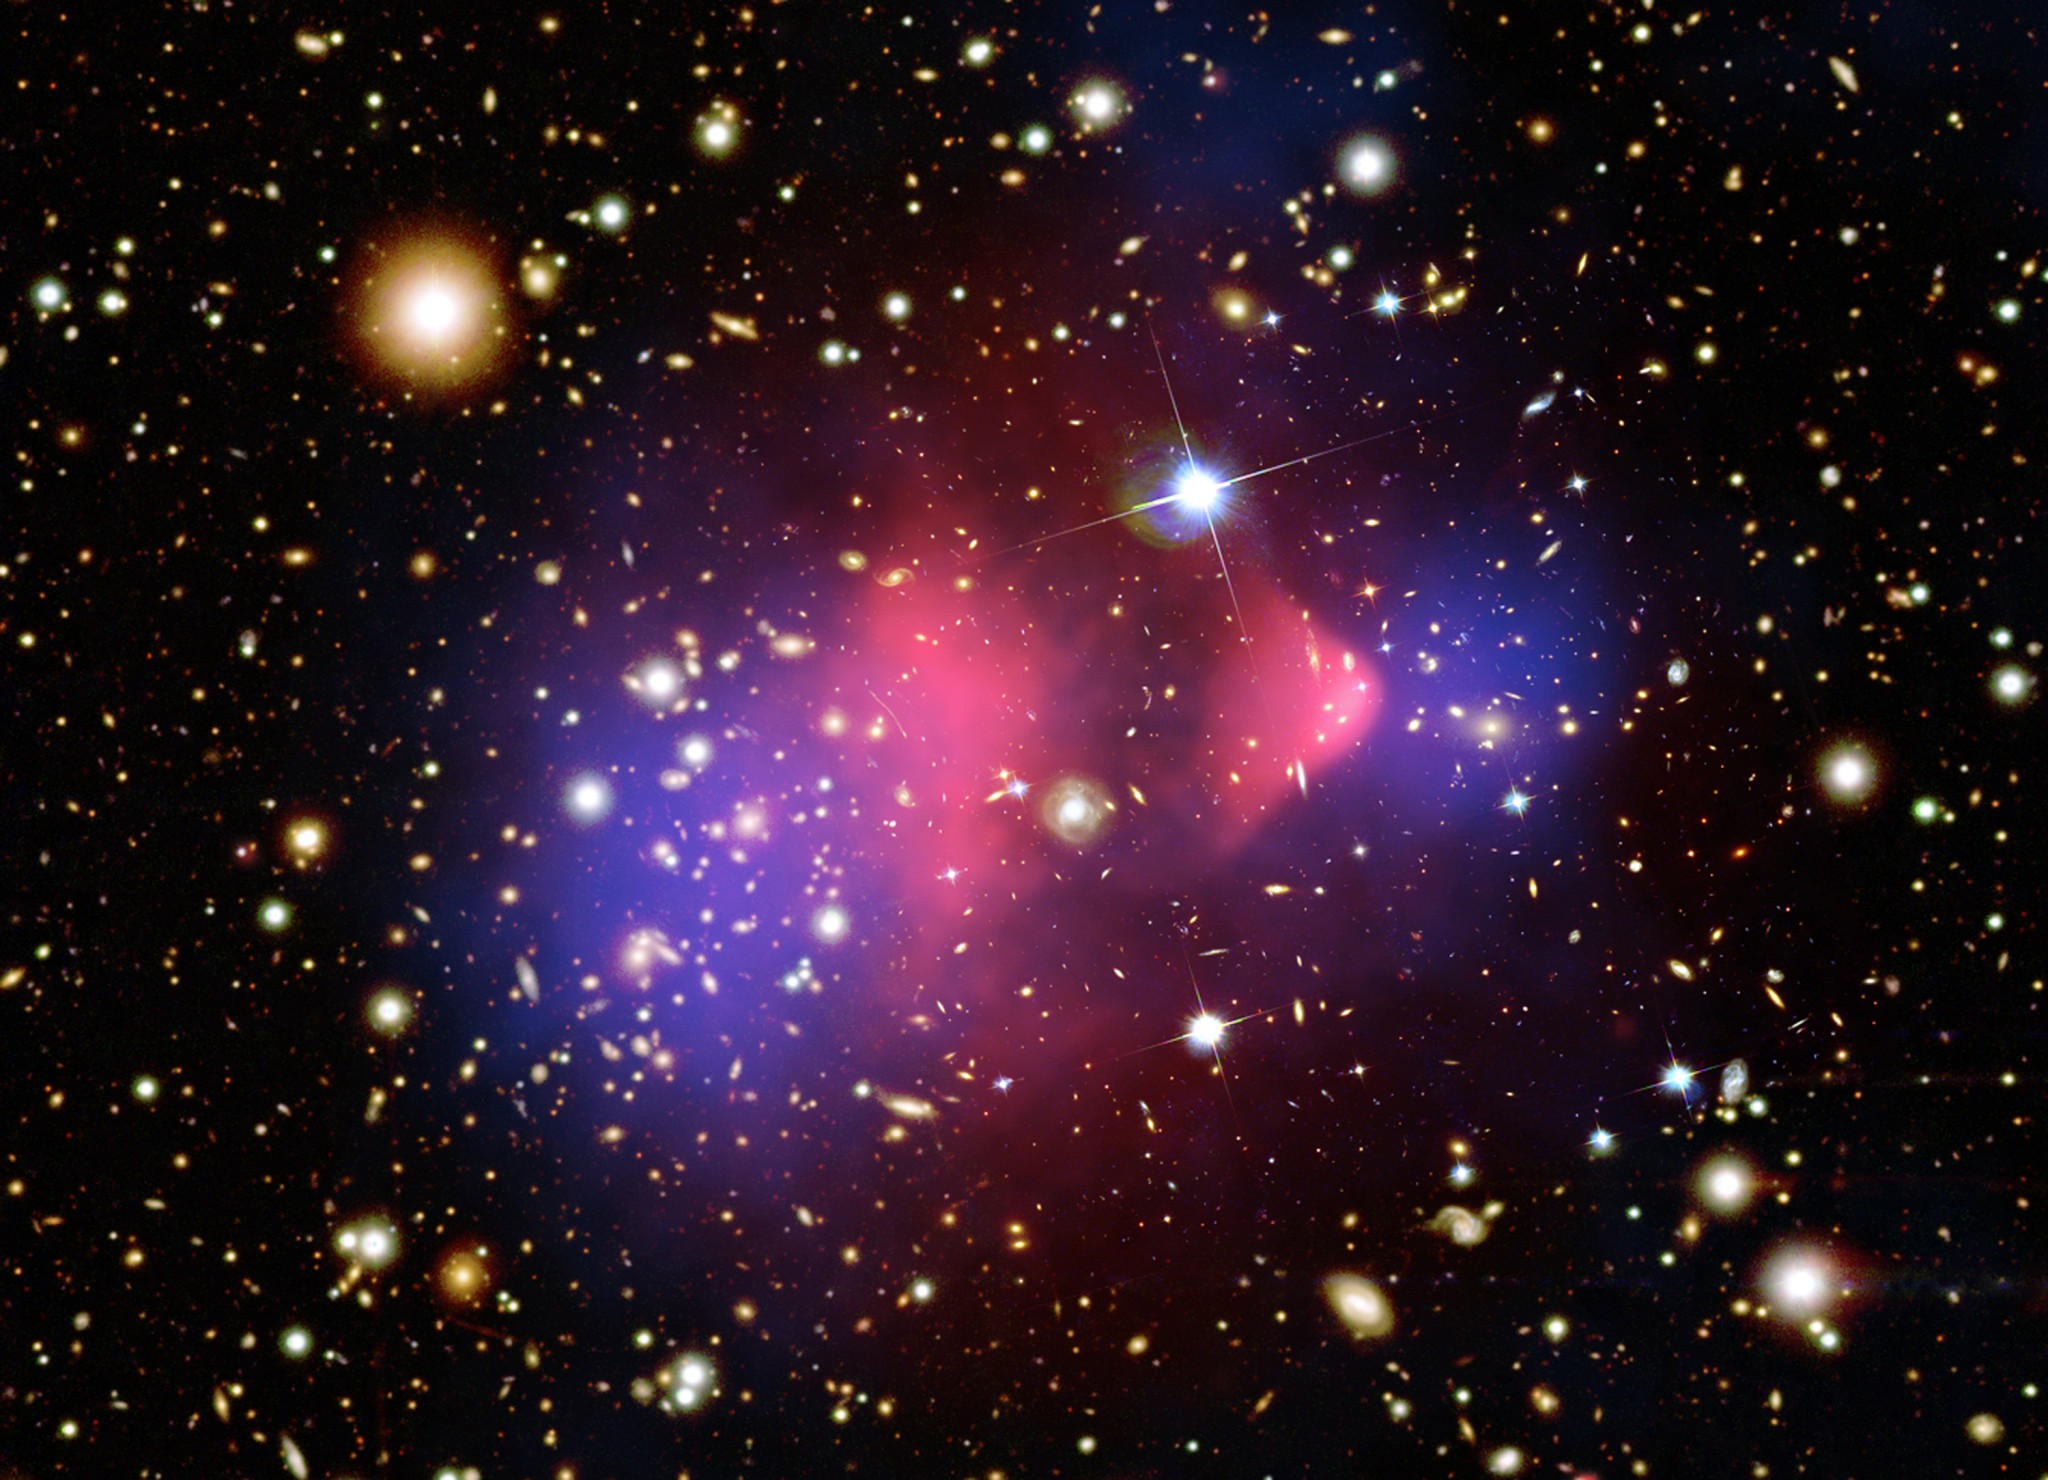
\includegraphics[width=0.8\textwidth]{bulletcluster}
      \end{figure}
      \vspace{-25pt}
      \begin{center}
        {\tiny [\href{https://apod.nasa.gov/apod/ap060824.html}{APOD/NASA}]} \\
        Dark matter?
      \end{center}
      \vspace{-15pt}
      \begin{figure}
        \centering
        \includegraphics[width=0.8\textwidth]{SM_gauge_rgflow}
      \end{figure}
      \vspace{-25pt}
      \begin{center}
        {\tiny [\href{http://flexiblesusy.hepforge.org/images.html}{%
        http://flexiblesusy.hepforge.org/images.html}]} \\
        Gauge unification?
      \end{center}
    \end{column}
    \begin{column}{0.7\textwidth}
      \begin{columns}[t]
        \begin{column}{0.5\textwidth}
          \vspace*{-30pt}
          \begin{figure}
            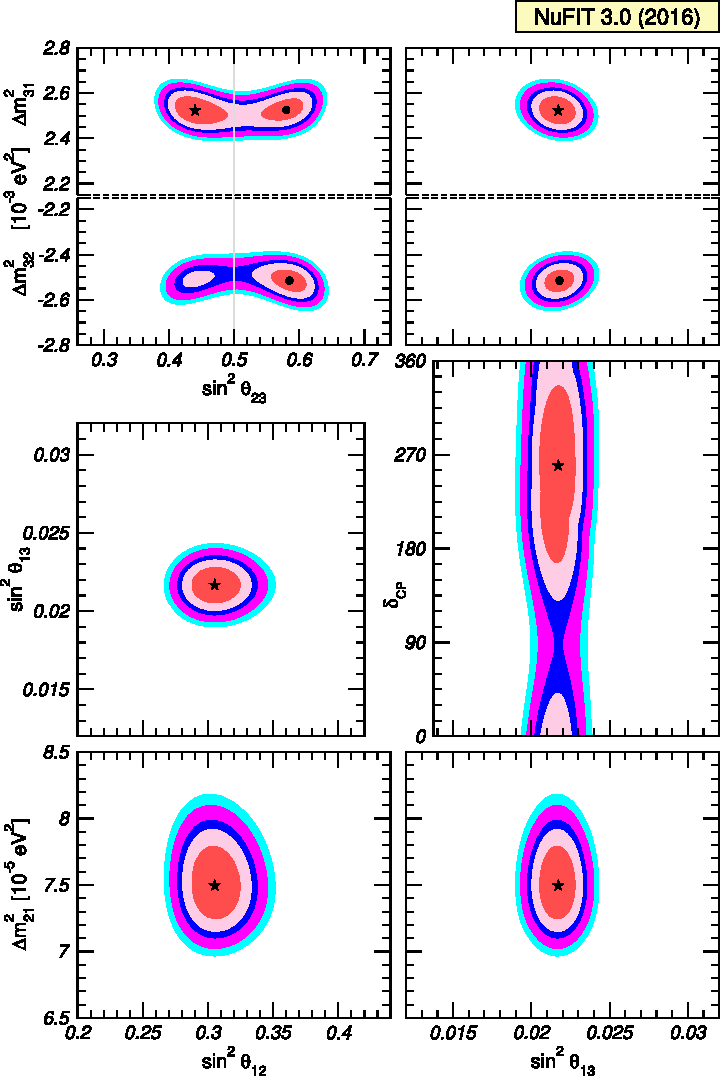
\includegraphics[width=0.85\textwidth]{neutrino_masses} \\
          \end{figure}
          \vspace*{-25pt}
          \begin{center}
            {\tiny [\href{https://arxiv.org/abs/1611.01514}{%
              arXiv:1611.01514}]} \\
            Neutrino masses?
          \end{center}
        \end{column}
        \begin{column}{0.5\textwidth}
          \begin{figure}
            \includegraphics[width=0.9\textwidth]{fermionloop}
          \end{figure}
          \begin{center}
            \alert{i.e., the "Hierarchy Problem"?}
          \end{center}
        \end{column}
      \end{columns}
    \end{column}
    \end{columns}
\end{frame}

% No-go theorems
%  - current understanding of QFT: characterised
%    by external spacetime symmetries and internal
%    (gauge) symmetries
%  - natural question: possible to describe by a
%    single unified symmetry group
%  - answer: no, due to CM (describe)
\begin{frame}
  \frametitle{The Coleman-Mandula Theorem}
  \begin{itemize}\itemsep1em
  \item Structure of SM: Poincar\'{e} $\times G_{SM}$
  \item {\color{blue} Idea: unify within continuous group $\mathcal{G}$?}
  \item E.g., consider conserved $Q_{\mu\nu}$ traceless, symmetric,
    \begin{equation*}
      \Rightarrow \langle p | Q_{\mu\nu} | p \rangle \propto p_\mu p_\nu
      - \frac{1}{d} \eta_{\mu\nu} p^2
    \end{equation*}
  \item Elastic scattering $p_1^\mu + p_2^\mu = q_1^\mu + q_2^\mu$,
    \begin{equation*}
      \langle p_1, p_2 | Q_{\mu\nu} | p_1, p_2 \rangle
      = \langle q_1, q_2 | Q_{\mu\nu} | q_1, q_2 \rangle
      \Rightarrow
      p_1^\mu p_1^\nu + p_2^\mu p_2^\nu = q_1^\mu q_1^\nu + q_2^\mu q_2^\nu
    \end{equation*}
  \item Solution: $p_1^\mu = q_1^\mu$ or $p_1^\mu = q_2^\mu$, \alert{i.e.,
    no scattering}
  \item Consequence of {\color{blue} Coleman-Mandula theorem} [1]
  \end{itemize}
      {\tiny [1] S.~Coleman and J.~Mandula,
        \href{http://dx.doi.org/10.1103/PhysRev.159.1251}{%
          Phys.~Rev.~\textbf{159} (1967) 1251} }
\end{frame}

\begin{frame}
  \frametitle{The Coleman-Mandula Theorem}
  Let $\mathcal{G}$ be a connected symmetry group of the $S$-matrix
  containing a subgroup locally isomorphic to the Poincar\'{e} group,
  $\mathcal{P}$.  Suppose that
    \begin{enumerate}\itemsep1em
    \item All particle types correspond to positive-energy representations
      of $\mathcal{P}$.  For any finite $M$, $\exists$ only a finite number
      of particle types with mass $m < M$
    \item Elastic scattering amplitudes are analytic functions of $s$, $t$,
      in some neighbourhood of the physical region, except at normal
      thresholds
    \item Let $|p \rangle$, $| p^\prime \rangle$ be any two 1-particle
      momentum eigenstates, $|p, p^\prime \rangle$ be the 2-particle state
      made from these.  Then
      \begin{equation*}
        T|p, p^\prime\rangle \neq 0
      \end{equation*}
      except perhaps for certain isolated values of $s$
    \item $\mathcal{G}$ is locally generated by generators represented by
      integral operators in momentum space with distributions as kernels
    \end{enumerate}
    Then $\mathcal{G}$ is locally isomorphic to $\mathcal{P} \times G$
\end{frame}

% Evading CM theorem
%  - can do so by violating assumption of only
%    bosonic generators, i.e., extend to graded
%    symmetry algebra
%  - HLS => SUSY is essentially unique such extension
%  - number of odd generators not restricted, but
%    focus on N = 1 SUSY (most relevant for TeV-scale
%    SUSY phenomenology)
\begin{frame}
  \frametitle{The HLS Theorem}
\end{frame}

% Super-Poincare algebra
%  - consequences: superpartners differ
%    in spin by 1/2, mass degeneracy
\begin{frame}
  \frametitle{The Super-Poincar\'{e} Algebra}
\end{frame}

\begin{frame}
  \frametitle{Implications of Global SUSY}
\end{frame}

% Local SUSY and supergravity
%  - very briefly, local SUSY => diffeomorphism invariance
%  - generalities of supergravity, but not details
\begin{frame}
  \frametitle{Local SUSY}
\end{frame}

% Hierarchy problem
%  - SUSY invariance => number of bosonic and fermionic
%    degrees of freedom must match (prove if space)
%  - in particular, all scalar degrees of freedom
%    associated with fermionic superpartners
%  - ensures scalar masses are symmetry protected from
%    quadratically divergent corrections (analogous to
%    chiral symmetry)
%  - relevance? SM contains a fundamental scalar, the Higgs,
%    soon realised that this should mix with heavy states
%    - known as the Hierarchy problem
%    - unbroken SUSY ``naturally'' cancels these divergent
%      corrections
\begin{frame}
  \frametitle{The Hierarchy Problem}
\end{frame}

% basic SUSY model building
\section{Basics of SUSY Model Building}

\begin{frame}
  \frametitle{Constructing SUSY Gauge Theories}
  \begin{block}{Example: Wess-Zumino Model [1]}
    \begin{equation*}
      \mathcal{L}_{WZ} = \partial^\mu \phi^\dagger \partial_\mu \phi
      + i \bar{\psi} \bar{\sigma}^\mu \partial_\mu \psi + {\color{red}
        F^\dagger F} + \left [ -\frac{m}{2} \psi \psi - \frac{y}{2} \phi \psi
        \psi + \left ( L + m \phi + \frac{y}{2} \phi^2 \right ) {\color{red} F}
        + h.c. \right ]
    \end{equation*}
    Global SUSY transformation $\Rightarrow$
    $\delta \phi = \sqrt{2} \epsilon \psi$,
    $\delta \psi_\alpha = \sqrt{2} \epsilon_\alpha F - i \sqrt{2}
    ( \sigma^\mu \bar{\epsilon})_\alpha \partial_\mu \phi$,
    $\delta F = -i \sqrt{2} \bar{\epsilon} \bar{\sigma}^\mu \partial_\mu \psi$.
  \end{block}
  \begin{itemize}\itemsep1em
  \item \emph{In principle}, can construct any SUSY model in terms of
    ``component fields''
  \item But:
    \begin{itemize}\itemsep0.5em
    \item Transformation properties (e.g., of $\phi$, $\psi$, $F$ in WZ model)
      and SUSY invariance \alert{are not obvious}
    \item SUSY $\Rightarrow$ \alert{non-trivial constraints on field
      content, interaction terms}
    \item Close SUSY algebra on- and off-shell $\Rightarrow$ \alert{auxiliary
      fields} ({\color{red} $F$})
    \end{itemize}
  \item {\color{blue} Better: formulate theory in language in which
    SUSY invariance is manifest}
  \end{itemize}
  \vfill
      { \tiny [1] J.~Wess and B.~Zumino,
        \href{http://dx.doi.org/10.1016/0550-3213(74)90355-1}{%
          Nucl.~Phys.~B \textbf{70} (1974) 39.}}
\end{frame}

% Superspace formalism
%  - certainly introduce basics sufficient for N = 1 SUSY,
%    i.e., extend x -> (x, \theta, \bar{\theta})
%  - how technical to go?
%  - ordinary functions -> superfields, i.e., functions defined
%    on superspace
%  - general Lorentz scalar superfield can be written as a
%    terminating power series in the anticommuting variables
%  - (global) SUSY realised as rigid translations on superspace
\begin{frame}
  \frametitle{Superspace and Superfields}
  \begin{columns}[t]
    \begin{column}{0.5\textwidth}
      \begin{itemize}\itemsep1em
      \item {\color{blue} Natural and compact} technique for constructing
        SUSY models:
      \end{itemize}
      \vspace*{5pt}
      \begin{figure}
        \centering
        \includegraphics[width=0.7\textwidth]{%
          supergauge_transformations_title}
      \end{figure}
      \vspace*{-2pt}
      \begin{tikzpicture}
        \node[draw, fill = white, rounded corners = 6pt,
          blur shadow = {shadow blur steps = 5}]{%
          \includegraphics[width=\textwidth]{%
            supergauge_transformations_quote}
          };
      \end{tikzpicture}
    \end{column}
    \begin{column}{0.5\textwidth}
      \begin{itemize}\itemsep1em
      \item Minkowski space $\to$ ($d = 4$, $N = 1$) Minkowski superspace:
        \begin{gather*}
          x^\mu \to z^A \equiv
          (x^\mu, \theta^\alpha, \bar{\theta}_{\dot{\alpha}} ), \\
          \{ \theta^\alpha, \theta^\beta \} =
          \{ \bar{\theta}_{\dot{\alpha}}, \bar{\theta}_{\dot{\beta}} \} =
          \{ \theta^\alpha , \bar{\theta}_{\dot{\beta}} \} = 0
        \end{gather*}
      \item Elements of super-Poincar\'{e} group
        \begin{equation*}
          g = \exp \left [ i \left ( \alpha^\mu \hat{P}_\mu
            - \frac{1}{2} \omega^{\mu \nu} \hat{M}_{\mu \nu}
            + \epsilon \hat{Q} + \bar{\epsilon} \hat{\bar{Q}} \right )
            \right ]
        \end{equation*}
      \item Global/rigid SUSY transformations $\Rightarrow$ {  \color{blue}
        translations in superspace},
        \begin{gather*}
          x^\mu \to x^\mu - i \theta \sigma^\mu \bar{\epsilon}
          + i \epsilon \sigma^\mu \bar{\theta} , \\
          \theta^\alpha \to \theta^\alpha + \epsilon^\alpha , \quad
          \bar{\theta}_{\dot{\alpha}} \to \bar{\theta}_{\dot{\alpha}} +
          \bar{\epsilon}_{\dot{\alpha}}
        \end{gather*}
      \end{itemize}
    \end{column}
  \end{columns}
\end{frame}

% - mention R-symmetry anywhere?

% Representations of SUSY
%  - most general such superfield is reducible
%  - relevant for N = 1 model building: chiral
%    superfields,  give definition and supermultiplet
%    structure (including auxiliary fields)
%  - vector superfields, give definition and
%    supermultiplet structure
\begin{frame}
  \frametitle{Representations of SUSY}
  \begin{itemize}\itemsep1em
  \item Constructed in terms of superfields $\equiv$ functions on superspace,
    e.g.,
    \begin{equation*}
      \hat{S}(z) = a(x) + \theta \xi(x) + \bar{\theta} \bar{\chi}(x) +
      \theta \theta b(x) + \bar{\theta} \bar{\theta} c(x) + \bar{\theta}
      \bar{\sigma}^\mu \theta v_\mu (x)
      + \bar{\theta} \bar{\theta} \theta \zeta(x)
      + \theta \theta \bar{\theta} \bar{\lambda} (x) + \frac{1}{2} \theta
      \theta \bar{\theta} \bar{\theta} d(x)
    \end{equation*}
  \item Coefficients $a$, $b$, $\ldots$, $\xi$, $\bar{\chi}$, $\ldots$
    $\Rightarrow$ component fields of \emph{supermultiplet} (16 real d.o.f)
  \item Action of SUSY generators on (scalar) superfield
    \begin{gather*}
      \delta_\epsilon S = i \left [ \epsilon \hat{Q} + \bar{\epsilon}
        \hat{\bar{Q}}, S \right ]
      = i \left ( \epsilon Q + \bar{\epsilon} \bar{Q} \right ) S ,
      \\
      Q_\alpha = -i \left [ \frac{\partial}{\partial \theta^\alpha}
        + i \left ( \sigma^\mu \bar{\theta} \right )_\alpha
        \partial_\mu \right ] , \quad
      \bar{Q}^{\dot{\alpha}} = -i \left [
        \frac{\partial}{\partial \bar{\theta}_{\dot{\alpha}}} + i \left (
        \bar{\sigma}^\mu \theta \right )^{\dot{\alpha}} \partial_\mu \right ]
    \end{gather*}
    $\Rightarrow$ transformation laws for component fields
  \item General superfield is a \alert{reducible representation of SUSY}
  \end{itemize}
\end{frame}

\begin{frame}
  \frametitle{The Chiral Supermultiplet}
  \begin{itemize}\itemsep1em
  \item Constrain general superfield $\Rightarrow$ {\color{blue} irreducible
    representations of SUSY}
  \item Introduce chiral covariant derivatives:
    \begin{equation*}
      \mathcal{D}_\alpha = \frac{\partial}{\partial \theta^\alpha}
      - i \left (\sigma^\mu \bar{\theta} \right )_\alpha \partial_\mu , \quad
      \bar{\mathcal{D}}^{\dot{\alpha}} = \frac{\partial}
          {\partial \bar{\theta}_{\dot{\alpha}}}  - i \left ( \bar{\sigma}^\mu
            \theta \right )^{\dot{\alpha}} \partial_\mu
    \end{equation*}
  \item Impose $\bar{\mathcal{D}}_{\dot{\alpha}} \Phi = 0$ $\Rightarrow$ $\Phi
    \equiv$ {\color{blue} left chiral superfield} (similarly,
    $\mathcal{D}_\alpha \Phi^\dagger = 0$ $\Rightarrow$ right chiral
    superfield)
  \item Solve constraint $\Rightarrow$ obtain component field description
    of chiral supermultiplet
  \end{itemize}
  \begin{block}{Left chiral supermultiplet}
    \begin{equation*}
      \Phi = \phi(x) - i \theta\sigma^\mu\bar{\theta} \partial_\mu
      \phi(x) - \frac{1}{4} \theta\theta\bar{\theta}\bar{\theta} \partial^\mu
      \partial_\mu \phi(x) + \sqrt{2} \theta \psi(x)
      + \frac{i}{\sqrt{2}} \theta\theta
      \partial_\mu \psi(x)\sigma^\mu \bar{\theta} + \theta \theta F(x)
    \end{equation*}
    with component fields $\phi$, $\psi$, $F$ (i.e., 4 real scalar, 4
    real fermion d.o.f)
  \end{block}
\end{frame}

\begin{frame}
  \frametitle{The Vector Supermultiplet}
  \begin{itemize}
  \item Defined by condition $V = V^\dagger$ $\Rightarrow$
    \begin{align*}
      V(z) &= C(x) + \sqrt{2} \theta \xi(x) + \bar{\theta} \bar{\xi}(x)
      + \theta \theta M(x) + \bar{\theta} \bar{\theta} M^*(x) +
      \theta \sigma^\mu\bar{\theta}A_\mu(x) \\
      & \quad {} + \theta\theta \bar{\theta}
      \left [ \bar{\lambda}(x) - \frac{i}{\sqrt{2}} \bar{\sigma}^\mu\partial_\mu
        \xi(x) \right ]
        + \bar{\theta} \bar{\theta} \theta \left [ \lambda(x)
        - \frac{i}{\sqrt{2}} \sigma^\mu \partial_\mu \bar{\xi}(x) \right ]
      + \theta\theta \bar{\theta}\bar{\theta} \left [ \frac{1}{2} D(x) -
        \frac{1}{4} \partial^\mu\partial_\mu C(x) \right ]
    \end{align*}
  \item Extra auxiliary fields $C$, $M$, $\xi$ eliminated via supergauge
    transformation, e.g.,
    \begin{equation*}
      V \to V + i ( \Lambda - \Lambda^\dagger ) , \quad \text{ where } \Lambda
      = \text{chiral superfield}
    \end{equation*}
  \item NB still have ability to carry out ordinary gauge transformations
  \end{itemize}
  \begin{block}{Vector supermultiplet (WZ gauge)}
    \begin{equation*}
      V_{WZ}(z) = \theta \sigma^\mu \bar{\theta} A_\mu(x) + \theta \theta
      \bar{\theta} \bar{\lambda}(x) + \bar{\theta} \bar{\theta} \theta
      \lambda(x) + \frac{1}{2} \theta\theta\bar{\theta}\bar{\theta} D(x)
    \end{equation*}
    with component fields $A_\mu$, $\lambda$, $D$ (4 real scalar, 4 real
    fermion d.o.f.)
  \end{block}
\end{frame}

% SUSY Lagrangians
% - construction of globally SUSY invariant actions
% - introduce notions of integration on superspace
% - introduce definitions of F- and D-terms of superfield
% - interactions amongst chiral superfields characterised
%   by superpotential
% - usual kinetic terms etc. appropriately generalised to
%   be supergauge invariant
\begin{frame}
  \frametitle{Global SUSY Invariant Actions}
  \begin{itemize}\itemsep1em
  \item Component field transformation properties:
    \begin{equation*}
      \delta F = -i \sqrt{2} \bar{\epsilon} \bar{\sigma}^\mu \partial_\mu \psi ,
      \quad \delta D = {\color{red} \text{TO DO}}
    \end{equation*}
  \item $\theta \theta$ component of chiral supermultiplet
    can contribute to SUSY invariant action $\Rightarrow$ {\color{blue}
      ``$F$-term'' contribution}
  \item Similarly $\theta\theta\bar{\theta}\bar{\theta}$ component
    from vector supermultiplet $\Rightarrow$ {\color{blue} ``$D$-term''
      contribution}
  \item Berezin integral satisfying translation invariance and linearity:
    \begin{equation*}
      \int d\theta \, (f_0 + \theta f_1) = f_1 , \quad
      \int d^2 \theta \, \theta \theta = 1 , \quad
      \int d^2 \bar{\theta} \, \bar{\theta} \bar{\theta} = 1 \quad
      \left [ \text{note } \Rightarrow \frac{d f}{d\theta} = \int d\theta\,
        f \right ]
    \end{equation*}
  \item Then build action out of contributions of form
    ($d^4\theta \equiv d^2 \bar{\theta} d^2 \theta$,
    $\delta^{(2)}(\bar{\theta}) \equiv \bar{\theta} \bar{\theta}$ )
    \begin{equation*}
      \left [ V \right ]_D \equiv \int d^4\theta \, V , \quad
      \left [ \Phi \right ]_F \equiv \int d^4 \theta \, \delta^{(2)}(
      \bar{\theta}) \Phi
    \end{equation*}
  \end{itemize}
\end{frame}

\begin{frame}
  \frametitle{Superspace Formulation of the Wess-Zumino Model}
  \begin{itemize}\itemsep1em
  \item $\phi$, $\psi$, $F$ $\to$ component fields of single chiral
    supermultiplet $\Phi$
  \item Obtain kinetic terms from $D$-term:
    \begin{equation*}
      \left [ \Phi^\dagger \Phi \right ]_D = \partial^\mu \phi^\dagger
      \partial_\mu \phi + i \bar{\psi} \bar{\sigma}^\mu \partial_\mu \psi
      + F^\dagger F ( + \text{ total derivative})
    \end{equation*}
  \item Interaction terms from $F$-term of {\color{blue} superpotential}:
    \begin{equation*}
      \left [ W(\Phi) \right ]_F = \left [ L \Phi + \frac{m}{2} \Phi^2
        + \frac{y}{6} \Phi^3 \right ]_F
      = -\frac{m}{2} \psi \psi - \frac{y}{2} \phi \psi \psi
      + (L + m \phi + \frac{y}{2} \phi^2) F
    \end{equation*}
    \item Full WZ Lagrangian:
      \begin{equation*}
        \mathcal{L}_{WZ} = \left [ \Phi^\dagger \Phi \right ]_D
        + \left [ W(\Phi) + h.c. \right ]_F
      \end{equation*}
    \item Find scalar potential $V = F^\dagger F \geq 0$, eliminate
      $F$ on-shell using EoM:
      \begin{equation*}
        F^\dagger = - \left . \frac{\partial W}{\partial \Phi} \right |_{\theta
          = \bar{\theta} = 0}
      \end{equation*}
  \end{itemize}
\end{frame}

% summarise standard form of invariant Lagrangian for
% non-Abelian SUSY gauge theory to which can refer
% back to
% - briefly mention also form for non-renormalisable models
%   relevant for discussion of SUGRA? may not be space
\begin{frame}
  \frametitle{Recipe for SUSY Models}
  \begin{block}{SUSY Gauge Theory}
    Given gauge group $G$, vector supermultiplet $V$, and chiral superfields
    $\Phi^I$ transforming under $G$,
    \begin{equation*}
      \mathcal{L} = \left [ \Phi^\dagger_I (e^V)^I{}_J \Phi^J \right ]_D
      + \frac{1}{16 k^2 g^2} \Tr \left [ \mathcal{W} \mathcal{W}
        + \bar{\mathcal{W}} \bar{\mathcal{W}} \right ]_F
      + \left [ W(\Phi^I) + h.c. \right ]_F
    \end{equation*}
  \end{block}
  \begin{itemize}\itemsep1em
  \item Gauge field strengths generalised by (note $k = $ Dynkin index)
    \begin{equation*}
      \mathcal{W}_\alpha = -\frac{1}{4} \bar{\mathcal{D}} \bar{\mathcal{D}}
      \left ( e^{-V} \mathcal{D}_\alpha e^V \right ) , \quad
      \bar{\mathcal{W}}^{\dot{\alpha}} = -\frac{1}{4} \mathcal{D} \mathcal{D}
      \left ( e^V \bar{\mathcal{D}}^{\dot{\alpha}} e^{-V} \right )
    \end{equation*}
  \item Renormalisable, gauge invariant superpotential
    \begin{equation*}
      W(\Phi^I) = \frac{1}{6} Y_{IJK} \Phi^I \Phi^J \Phi^K
      + \frac{1}{2} \mu_{IJ} \Phi^I \Phi^J + L_I \Phi^I
    \end{equation*}
  \item Scalar potential
    \begin{equation*}
      {\color{blue} V(\phi^I, \phi^\dagger_I) = F^\dagger_I F^I
        + \frac{1}{2} D^a D^a
      \geq 0 }, \quad
      F^I = \left . -\frac{\partial W^\dagger}{\partial \Phi^\dagger_I}
      \right |_{\theta = \bar{\theta} = 0} , \quad
      D^a = -g \phi^\dagger_I (T^a)^I{}_J \phi^J
    \end{equation*}
  \end{itemize}
\end{frame}

% SUSY breaking
% - empirically SUSY must be broken
% - broken SUSY still avoids quadratic divergences
%   provided softly broken
% - part of definining SUSY model => defining SUSY
%   breaking mechanism
% - explicit or spontaneous breaking,
%   ``top-down'' or ``bottom-up'' approach?
% - basic details of spontaneous SUSY breaking and
%   simplest examples, e.g. Planck mediated (permits
%   later introduction of CMSSM, CNMSSM, CE6SSM)
%     - only mention but do not give details of GMSB, AMSB etc.
% - ultimately, mechanism of high-scale SUSY breaking
%   (if it exists) remains unknown => for phenomenological
%   investigations write down (almost) most general
%   set of soft SUSY breaking interactions
%      - summarise, i.e., soft scalar masses, trilinears,
%        gaugino massses
\begin{frame}
  \frametitle{(Soft) SUSY Breaking}
  \begin{columns}[t]
    \begin{column}{0.5\textwidth}
      \begin{itemize}\itemsep1em
      \item {\color{blue} SUSY Lagrangian specified in very elegant and
        economical fashion} $\ldots$
      \item $\ldots$ \alert{but empirically low-energy SUSY must be broken}
      \item $\Rightarrow$ any phenomenologically viable model must include a
        SUSY breaking sector
      \item Cancellation of quadratic divergences preserved
        provided SUSY only {\color{blue} softly broken} [2]
      \item Generate soft breaking interactions $\Rightarrow$
        SUSY spontaneously broken?
      \end{itemize}
    \end{column}
    \begin{column}{0.5\textwidth}
      \begin{center}
      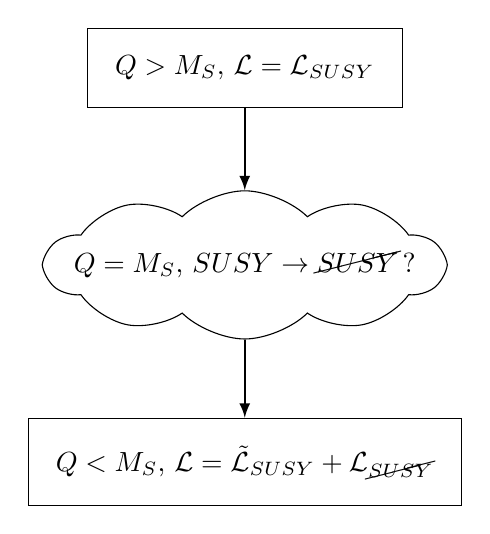
\begin{tikzpicture}[node distance=2.5cm, auto]
        \tikzstyle{arrow} = [draw, -latex, thick]

        \node[rectangle, draw, text centered, inner sep = 1em] (high scale)
             { $Q > M_S$, $\mathcal{L} = \mathcal{L}_{SUSY}$ };

        \node[cloud, draw, cloud puff arc = 90, aspect=4,
          below of = high scale, inner sep = -1em]
        (susy breaking) { $Q = M_S$, $SUSY \to \SUSYv\,$?};

        \node[rectangle, draw, text centered, below of = susy breaking,
        inner sep = 1em]
        (low scale)
             { $Q < M_S$,
               $\mathcal{L} = \tilde{\mathcal{L}}_{SUSY}
               + \mathcal{L}_{\SUSYv}$ };

        \path[arrow] (high scale) -- node {} (susy breaking);
        \path[arrow] (susy breaking) -- node {} (low scale);
      \end{tikzpicture}
      \end{center}
    \end{column}
  \end{columns}
      {\tiny [2] L.~Girardello and M.~T.~Grisaru,
        \href{http://dx.doi.org/10.1016/0550-3213(82)90512-0}{%
          Nucl.~Phys.~B \textbf{194} (1982) 65} }
\end{frame}

\begin{frame}
  \frametitle{Spontaneous SUSY Breaking}
  \begin{columns}[t]
    \begin{column}{0.5\textwidth}
      \begin{itemize}\itemsep1em
      \item \alert{Difficult!}
        \begin{itemize}
        \item Mass sum rule:
          \begin{equation*}
            \STr(m^2) = \sum_{\text{spins } j} (-1)^{2j} (2 j + 1) \Tr(m_j^2)
            = 0
          \end{equation*}
        \item $\Rightarrow$ superpartners of SM fields too light if only
          available SUSY breaking states
        \end{itemize}
      \item Break SUSY in hidden sector, transmit to visible sector via
        mediator interactions
      \item Super-Poincar\'{e} algebra $\Rightarrow$ SSB iff $\langle \Omega
        | H | \Omega \rangle \neq 0$
      \item $V \sim |F|^2 + |D|^2$ $\Rightarrow$ non-zero hidden sector $F$-
        (O'Raifeartaigh) or $D$-term (Fayet-Iliopoulos) VEV
      \end{itemize}
    \end{column}
    \begin{column}{0.5\textwidth}
      \begin{empheq}[box=\widefbox]{equation*}
        H = P^0 = \frac{1}{2} \left ( \{Q_1, \bar{Q}_{\dot{1}} \}
        + \{Q_2, \bar{Q}_{\dot{2}} \} \right )
      \end{empheq}
      \begin{center}
        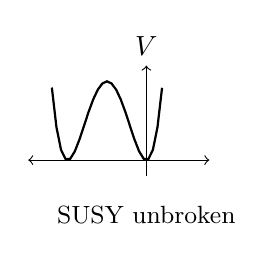
\begin{tikzpicture}[domain=-1.2:0.2]
          \draw[<->] (-1.5,0) -- (0.8,0) node {};
          \draw[->] (0,-0.2) -- (0,1.2) node[above] {$V$};
          \draw[thick] plot (\x, {16 * \x * \x * (\x + 1) * (\x + 1)}) node {};
          \node[draw = none, text centered] at (0, -0.7) { \small SUSY unbroken };
        \end{tikzpicture}
        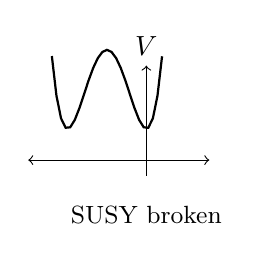
\begin{tikzpicture}[domain=-1.2:0.2]
          \draw[<->] (-1.5,0) -- (0.8,0) node {};
          \draw[->] (0,-0.2) -- (0,1.2) node[above] {$V$};
          \draw[thick] plot (\x, {16 * \x * \x * (\x + 1) * (\x + 1) + 0.4}) node {};
          \node[draw = none, text centered] at (0, -0.7) { \small SUSY broken };
        \end{tikzpicture}\\
        \vspace*{5pt}
        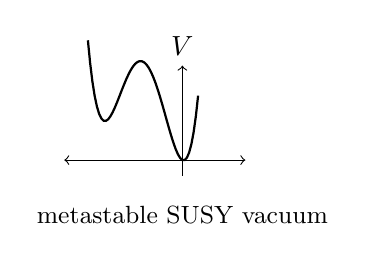
\begin{tikzpicture}[domain=-1.2:0.2, samples=50]
          \draw[<->] (-1.5,0) -- (0.8,0) node {};
          \draw[->] (0,-0.2) -- (0,1.2) node[above] {$V$};
          \draw[thick] plot (\x, {16 * \x * \x * (\x + 1) * (\x + 1) - 0.5 * \x})
          node {};
          \node[draw = none, text centered] at (0, -0.7)
               { \small metastable SUSY vacuum };
        \end{tikzpicture}
      \end{center}
    \end{column}
  \end{columns}
\end{frame}

\begin{frame}
  \frametitle{Example: Gravity-mediated SUSY Breaking}
  \begin{itemize}\itemsep1em
  \item Hidden sector ($X^I$) breaking $\to$ visible sector ($Z^I$) via
    gravitational strength interactions
    \begin{itemize}\itemsep0.5em
    \item Automatically present for local SUSY/SUGRA
    \item Breakdown of local SUGRA $\Rightarrow$ gravitino
      acquires mass $m_{3/2}$ via super-Higgs mechanism
    \end{itemize}
  \item SUGRA: $\Phi^\dagger \Phi \to$ K\"{a}hler potential
    $K(\Phi, \Phi^\dagger e^V)$, e.g.,
    \begin{equation*}
      K = Z^\dagger Z + \frac{1}{M_{Pl}} ( X + X^\dagger) Z^\dagger Z
      + \ldots
    \end{equation*}
  \item $\langle F_X \rangle \neq 0$ $\Rightarrow$ soft SUSY breaking
    interactions in visible sector
    \begin{equation*}
      -\mathcal{L}_{\text{soft}} = \frac{|\langle F_X \rangle|^2}{M_{Pl}^2}
      z^\dagger z + \left ( \frac{\langle F_X \rangle}{M_{Pl}} z \left .
      \frac{\partial W} {\partial Z} \right |_{\theta = \bar{\theta} = 0}
      + h.c. \right ) + \ldots
    \end{equation*}
  \item Realistic SUGRA models $\Rightarrow$ generate soft interactions
    \begin{equation*}
      -\mathcal{L}_{\text{soft}} = m_0^2 \phi^\dagger_I \phi^I + \left (
      \frac{1}{6} Y_{IJK} A_0 \phi^I \phi^J \phi^K + \frac{1}{2} \mu_{IJ}
      B_0 \phi^I \phi^J + S_I \phi^I + h.c. \right )
      + \frac{1}{2} \left ( M_{1/2} \lambda^a \lambda^a + h.c. \right ) ,
    \end{equation*}
    i.e., {\color{blue} soft interactions determined by universal $m_0^2$,
      $A_0$, $B_0$, $M_{1/2}$}, size related to $m_{3/2} \sim \langle F
    \rangle / M_{Pl}$
  \end{itemize}
\end{frame}

\begin{frame}
  \frametitle{The Bottom-up Approach}
  \begin{itemize}\itemsep1em
  \item \alert{Detailed mechanism of SSB is unknown, many alternatives proposed}
    (gravity mediated, GMSB, AMSB, $\ldots$)
  \item Alternative: break SUSY explicitly using (almost) most general
    set of soft interactions:
    \begin{equation*}
      -\mathcal{L}_{\text{soft}} =  (m^2)^I{}_J \phi^\dagger_I \phi^J +
      \left ( \frac{1}{6} a_{IJK} \phi^I \phi^J \phi^K
      + \frac{1}{2} b_{IJ} \phi^I \phi^J + S_I \phi^I
      + h.c. \right ) + \frac{1}{2} \left ( M^a \lambda^a \lambda^a + h.c.
      \right )
    \end{equation*}
  \item \alert{Standard but non-exhaustive set}: also Dirac gaugino masses
    $m^D_{Ia}\psi^I \lambda^a$,
    trilinears $r^I{}_{JK} \phi^\dagger_I \phi^J\phi^K$
  \item {\color{blue} Phenomenologically useful:} cover wide range of SUSY
    breaking scenarios $\ldots$
  \item $\ldots$ \alert{at cost of many new parameters}
  \item Note: underlying SSB model $\Rightarrow$ relations among soft
    breaking parameters (e.g., $(m^2)^I{}_J \to m_0^2 \delta^I_J$)
  \end{itemize}
\end{frame}

% MSSM
\section{The MSSM}

% - general formalism now applied to construct phenomenologically
%   viable SUSY models
% - basic idea: ``supersymmetrise'' the SM by taking the known
%   matter content and gauge symmetries and embedding appropriately
%   into chiral and vector supermultiplets
% - simple considerations show that all superpartners must be
%   new states (e.g., no colour adjoint fermions observed)
% - thus SM -> MSSM by promoting all gauge fields to individual vector
%   supermultiplets, all matter fields to chiral superfields
% - one further complication: holomorphic superpotential and anomaly
%   cancellation => need second Higgs doublet chiral superfield
% - summarise field content
\begin{frame}
  \frametitle{Requirements on a Realistic SUSY Model}
  \begin{block}{Aim}
    Extend SM to be consistent with global SUSY
  \end{block}
  \begin{itemize}\itemsep1em
  \item Embedding into supermultiplets?
    \begin{itemize}\itemsep0.5em
    \item SUSY commutes with $G_{SM}$
    \item $\Rightarrow$ superpartner of, e.g., gluon is colour octet fermion
    \item Combining, e.g., Higgs, lepton doublet into chiral multiplet
      excluded
    \item \alert{SUSY $\Rightarrow$ \emph{new} states in chiral, vector
      supermultiplets}
    \end{itemize}
  \item SM Yukawas $\to$ superpotential interactions
    \begin{itemize}\itemsep0.5em
    \item Complication: $W$ depends on $\Phi$ only, not $\Phi^\dagger$,
      mass terms for fermions?
    \item Spin-$1/2$ Higgs partners spoil anomaly cancellation
    \end{itemize}
  \item Recipe for SUSY gauge theory $\Rightarrow$ {\color{blue} model then
    characterised by superpotential and soft terms}
  \end{itemize}
\end{frame}

\begin{frame}
  \frametitle{The MSSM: A Schematic View}
  \begin{tabularx}{\textwidth}{VVV}
    \begin{tabular}{c}
    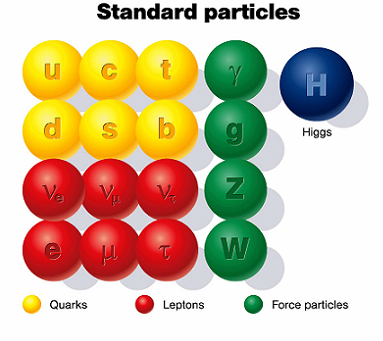
\includegraphics[width=0.25\textwidth]{susyparticles_sm_cropped} \\
    \phantom{\tiny Caption}
  \end{tabular} &
    \hspace{15pt}
    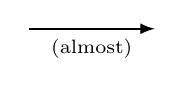
\begin{tikzpicture}
      \path[draw, -latex, thick] (-0.8,0) --node[below]  {\scriptsize (almost)} (0.8,0);
    \end{tikzpicture} &
    \begin{tabular}{c}
      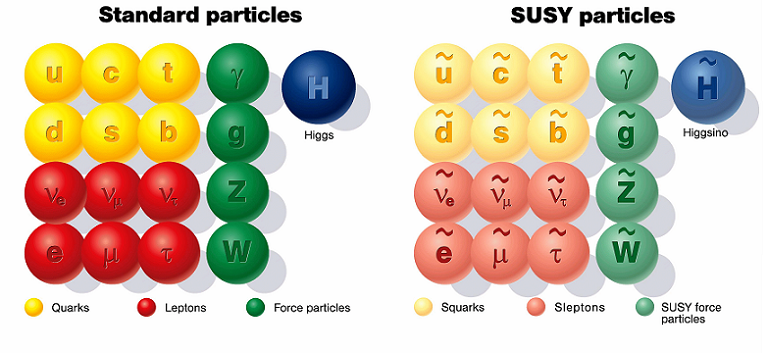
\includegraphics[width=0.5\textwidth]{susyparticles_sm} \\
      {\tiny [\href{http://www.physics.gla.ac.uk/ppt/bsm.htm}{%
      http://www.physics.gla.ac.uk/ppt/bsm.htm}] }
    \end{tabular}
  \end{tabularx}
  \vspace*{-70pt}
  \begin{tabular}{VVV}
    \includegraphics[width=0.25\textwidth]{fermionloop2} &
    \hspace{15pt}
    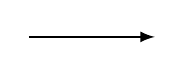
\begin{tikzpicture}
      \path[draw, -latex, thick] (-0.8,0) --node {} (0.8,0);
    \end{tikzpicture} &
    \begin{equation*}
      \parbox{20mm}{\includegraphics[width=0.2\textwidth]{fermionloop2}}
      \quad \quad \quad \, + \quad
      \parbox{20mm}{\includegraphics[width=0.2\textwidth]{scalarcubicloop} \\
        \vspace*{-5pt}
      \includegraphics[width=0.2\textwidth]{scalarquarticloop} }
    \end{equation*}
  \end{tabular}
  \vspace{90pt}
\end{frame}

\begin{frame}
  \frametitle{MSSM Field Content}
  \begin{table}[h]
    \centering
    \small
    \begin{tabular}{cccccc}
      \toprule
      & $s = 0$ & $s = \frac{1}{2}$ & $SU(3)_C$ & $SU(2)_L$
      & $\sqrt{\frac{5}{3}} Q_i^Y$ \\
      \midrule
      $Q_i$ & $\begin{pmatrix} \tilde{u}_{L} \\
        \tilde{d}_{L} \end{pmatrix}_i$
      & $\begin{pmatrix} u_{L} \\ d_L\end{pmatrix}_i$
        & $\mathbf{3}$ & $\mathbf{2}$ & $\frac{1}{6}$ \\[1em]
        $u^c_i$ & $\tilde{u}^*_{iR}$ & $u^c_{iR}$
        & $\bar{\mathbf{3}}$ & $\mathbf{1}$ & $-\frac{2}{3}$ \\[0.5em]
        $d^c_i$ & $\tilde{d}^*_{iR}$ & $d^c_{iR}$
        & $\bar{\mathbf{3}}$ & $\mathbf{1}$ & $\frac{1}{3}$ \\[0.5em]
        $L_i$ & $\begin{pmatrix} \tilde{\nu}_{L} \\
          \tilde{e}_{L} \end{pmatrix}_i$
        & $\begin{pmatrix} \nu_{L}\\ e_L \end{pmatrix}_i$
        & $\mathbf{1}$ & $\mathbf{2}$ & $-\frac{1}{2}$ \\[1em]
        $e^c_i$ & $\tilde{e}^*_{iR}$ & $e^c_{iR}$
        & $\mathbf{1}$ & $\mathbf{1}$ & $1$ \\[0.5em]
        $H_d$ & $\begin{pmatrix} H_d^0 \\ H_d^- \end{pmatrix}$
        & $\begin{pmatrix} \tilde{H}_d^0 \\ \tilde{H}_d^- \end{pmatrix}$
        & $\mathbf{1}$ & $\mathbf{2}$ & $-\frac{1}{2}$ \\[1em]
        $H_u$ & $\begin{pmatrix} H_u^+ \\ H_u^0 \end{pmatrix}$
        & $\begin{pmatrix} \tilde{H}_u^+ \\ \tilde{H}_u^0 \end{pmatrix}$
        & $\mathbf{1}$ & $\mathbf{2}$ & $\frac{1}{2}$ \\[1em]
        \bottomrule
    \end{tabular}
  \end{table}
\end{frame}

% - given matter content and symmetries, specification of SUSY
%   invariant part of MSSM completed by giving most general gauge
%   invariant and renormalisable superpotential, state
% - most general superpotential is dead on arrival due to too large
%   B and L violating interactions at tree-level
% - commonest scenario:rescue by imposing discrete R-parity
%   (discrete subgroup of U(1)_R symmetry, mention previously?)
% - structure of superpotential is reduced to only B and L conserving
%   interactions
\begin{frame}
  \frametitle{$R$-Parity in the MSSM}
  \vspace*{-5pt}
  \begin{block}{General MSSM superpotential}
    \begin{align*}
      W_{\text{MSSM}} &= \mu ( H_d \cdot H_u )
      + y_{ij}^e e^c_i ( L_j \cdot H_d )
      + y_{ij}^d d^c_i ( Q_j \cdot H_d )
      + y_{ij}^u u_i^c ( H_u \cdot Q_j ) \\
      & \quad {} {\color{red} - \epsilon_i L_i \cdot H_u
      + \frac{1}{2} \rho_{ijk} L_i \cdot L_j e_k^c
      + \rho^\prime_{ijk} L_i \cdot Q_j d_k^c
      + \frac{1}{2} \rho^{\prime\prime}_{ijk} u_i^c d_j^c d_k^c }
    \end{align*}
  \end{block}
  \vspace*{-10pt}
  \begin{columns}[t]
    \begin{column}{0.5\textwidth}
      \begin{itemize}
      \item Most general $W_{\text{MSSM}}$ $\Rightarrow$
        unacceptable $B$, $L$ violation
      \item Standard solution: impose {\color{blue} $R$-parity
        $\equiv$ matter parity}
        \begin{equation*}
          Z_2^R = (-1)^{3 (B - L) + 2 s}, \quad
          Z_2^M = (-1)^{3(B - L)}
        \end{equation*}
      \item Originate, e.g., as discrete subgroup of $U(1)_R$
        \begin{equation*}
          \theta \to e^{i \alpha \theta} , \quad \bar{\theta} \to
          e^{-i \alpha} \bar{\theta}
        \end{equation*}
        or, e.g., subgroup of gauged $U(1)$ (see later)
      \end{itemize}
    \end{column}
    \begin{column}{0.5\textwidth}
      \begin{figure}
        \includegraphics[width=0.5\linewidth]{protondecay}
      \end{figure}
    \end{column}
  \end{columns}
\end{frame}

% - mention variants of different soft Lagrangian, e.g., pMSSM, CMSSM
\begin{frame}
  \frametitle{The Constrained MSSM}
  \vspace*{-10pt}
  \begin{block}{Standard RPC soft terms}
    \begin{align*}
      -\mathcal{L}_{\text{MSSM}}^{\text{soft}} &=
      m_{Q_{ij}}^2 \tilde{Q}_i^\dagger \tilde{Q}_j + m_{u^c_{ij}}^2
      (\tilde{u}^c_i)^\dagger \tilde{u}^c_j + m_{d^c_{ij}}^2
      (\tilde{d}^c_i)^\dagger \tilde{d}^c_j + m_{L_{ij}}^2 \tilde{L}_i^\dagger
      \tilde{L}_j + m_{e^c_{ij}}^2 (\tilde{e}^c_i)^\dagger \tilde{e}^c_j
      + m_{H_u}^2 |H_u|^2 + m_{H_d}^2 |H_d|^2 \\
      & \quad {} + \left ( B\mu H_d \cdot H_u + h.c. \right )
      +  \left ( T^u_{ij}\tilde{u}_i^c H_{u} \cdot \tilde{Q}_j
      + T^d_{ij} \tilde{d}_i^c \tilde{Q}_j \cdot H_{d}
      + T^e_{ij} \tilde{e}_i^c \tilde{L} \cdot H_{d} + h.c. \right ) \\
      & \quad {}  + \frac{1}{2} \left ( M_1 \tilde{B} \tilde{B}
      + M_2 \tilde{W} \tilde{W} + M_3 \tilde{G} \tilde{G} + h.c. \right )
    \end{align*}
  \end{block}
  \vspace*{-10pt}
  \begin{columns}[t]
    \begin{column}{0.5\textwidth}
      \begin{columns}[t]
        \begin{column}{0.5\textwidth}
          \vspace*{5pt}
          \begin{figure}
            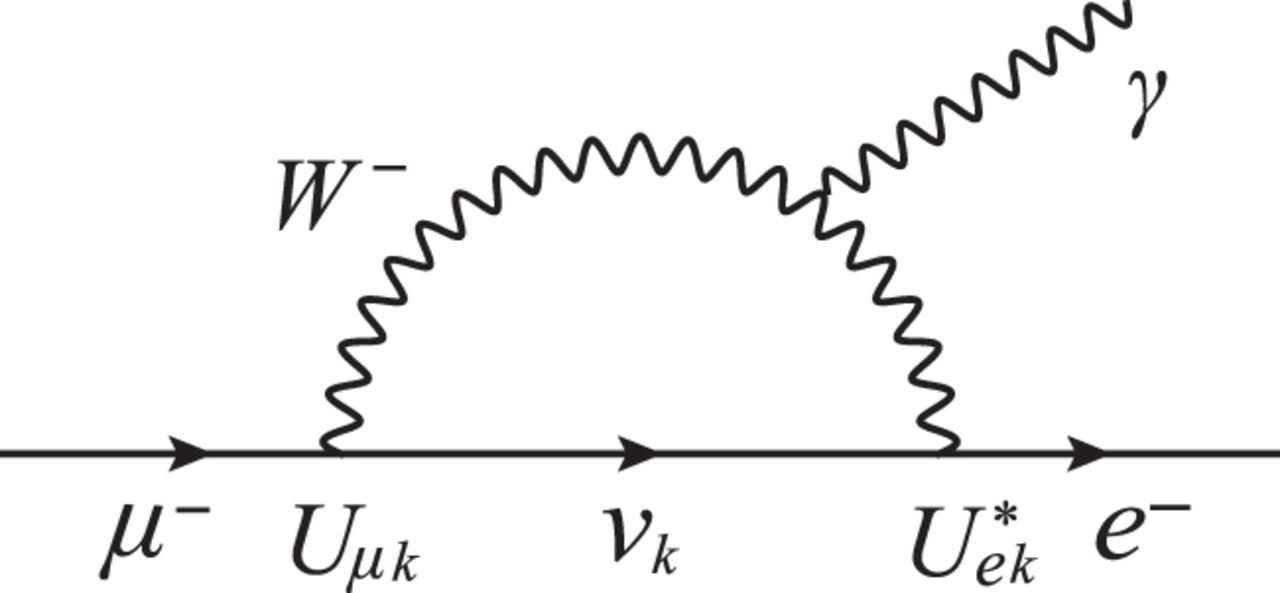
\includegraphics[width=\textwidth]{comet_sm_clfv}
          \end{figure}
        \end{column}
        \begin{column}{0.5\textwidth}
          \begin{figure}
            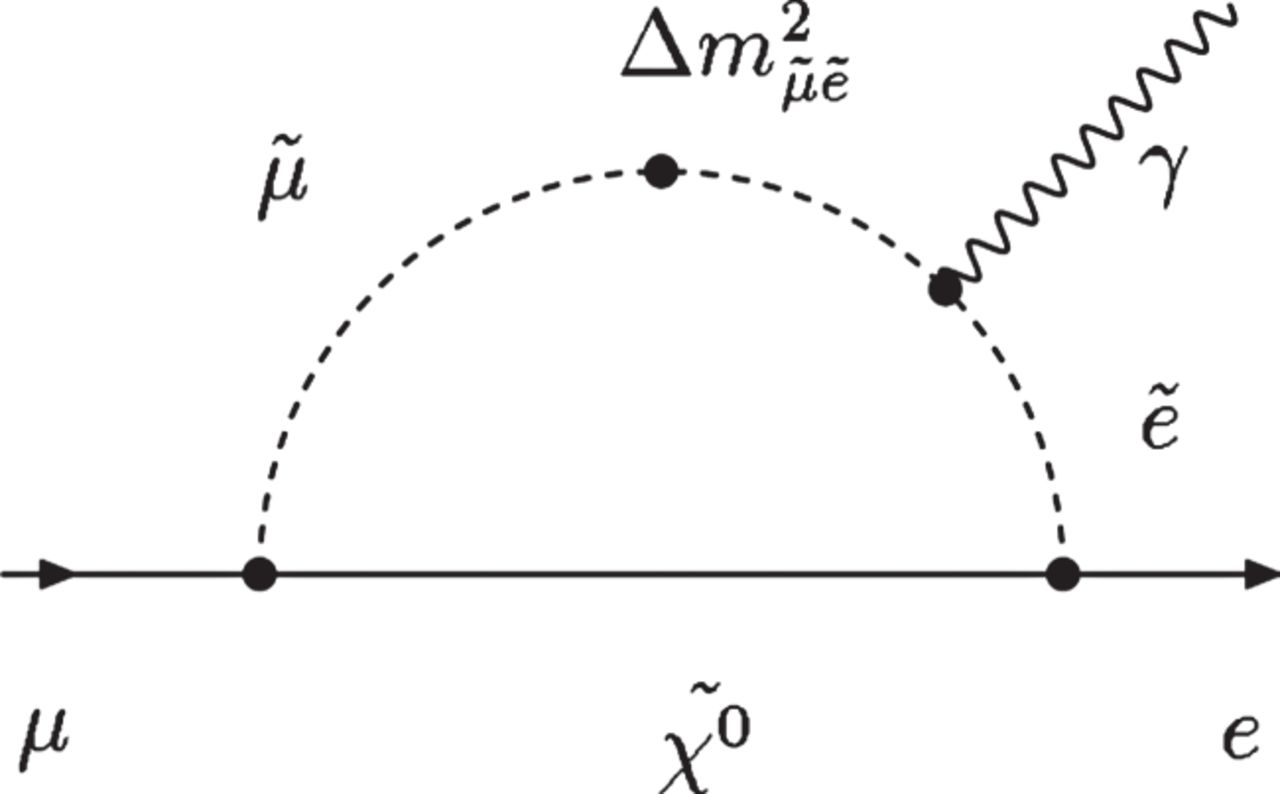
\includegraphics[width=0.9\textwidth]{comet_mssm_clfv}
          \end{figure}
      \end{column}
      \end{columns}
      \begin{center}
        { \tiny [\href{http://dx.doi.org/10.1093/ptep/pts089}{%
              COMET collaboration, PTEP \textbf{2013} (2013) 022C01}]
        }
      \end{center}
    \end{column}
    \begin{column}{0.5\textwidth}
      \begin{itemize}\itemsep1em
      \item MSSM SUSY sector: {\color{blue} 1 additional complex parameter
        $\mu$}
      \item With general soft terms: \alert{105 new parameters}
      \item SSB mechanism $\Rightarrow$ constraints? E.g., CMSSM:
        \begin{gather*}
          m_Q^2 = m_{u^c}^2 = m_{d^c}^2 = m_L^2 = m_{e^c}^2 = m_0^2 \bm{1} \\
          m_{H_d}^2 = m_{H_u}^2 = m_0^2, \quad
          T^{u,d,e} = y^{u,d,e} A_0 \bm{1} \\
          M_1 = M_2 = M_3 = M_{1/2}
        \end{gather*}
      \end{itemize}
    \end{column}
  \end{columns}
\end{frame}

% phenomenological consequences of the MSSM
% - superpartner spectrum
\begin{frame}
  \frametitle{The Sparticle Spectrum}
  \begin{columns}[t]
    \begin{column}{0.5\textwidth}
      \begin{figure}
        \centering
        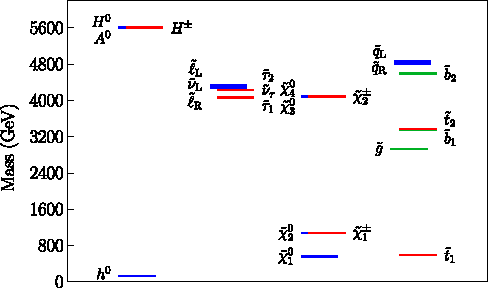
\includegraphics[width=0.9\textwidth]{gambit_cmssm_best_fit}
      \end{figure}
      \vspace*{-25pt}
      \begin{center}
        { \tiny [ \href{http://arxiv.org/abs/1705.07935}{%
              CMSSM, arXiv:1705.07935}] }
      \end{center}
      \begin{itemize}\itemsep1em
      \item Mass basis $\Rightarrow$ $u$-, $d$-type squarks ($\tilde{u}$,
        $\tilde{d}$), sleptons ($\tilde{l}$), EW-inos ($\tilde{\chi}^0$,
        $\tilde{\chi}^\pm$), gluino ($\tilde{g}$)
      \item {\color{blue} Extended Higgs sector}
      \end{itemize}
    \end{column}
    \begin{column}{0.5\textwidth}
      \vspace*{-15pt}
      \begin{itemize}\itemsep1em
      \item \alert{Spectrum (and $\therefore$ signatures) depends heavily
        on pattern of soft terms}
        \begin{itemize}
        \item Reconstruct soft masses? $\Rightarrow$ ``LHC inverse
          problem''
        \end{itemize}
      \item Some general features: $\tilde{\chi}^0$ LSP (or $\tilde{G}$),
        $m_{\tilde{g}} > m_{\tilde{\chi}^0}, m_{\tilde{\chi}^\pm}$, $\ldots$
      \end{itemize}
      \begin{figure}
        \centering
        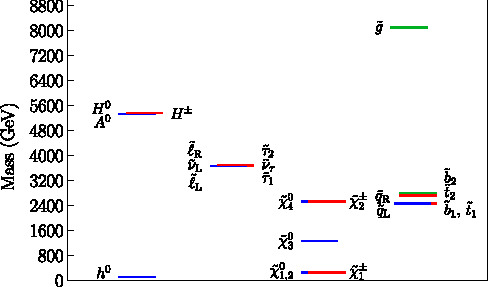
\includegraphics[width=0.9\textwidth]{gambit_mssm7_best_fit}
      \end{figure}
      \vspace*{-25pt}
      \begin{center}
        { \tiny [\href{http://arxiv.org/abs/1705.07917}{%
              MSSM7, arXiv:1705.07917}] }
      \end{center}
    \end{column}
  \end{columns}
\end{frame}

% - improved gauge unification, REWSB
\begin{frame}
  \frametitle{RG Evolution in the MSSM}
  \begin{columns}[t]
    \begin{column}{0.5\textwidth}
      \begin{figure}
        \centering
        \includegraphics[width=0.8\textwidth]{CMSSM_gauge_rgflow}
      \end{figure}
      \vspace{-25pt}
      \begin{center}
        {\tiny [\href{http://flexiblesusy.hepforge.org/images.html}{%
              http://flexiblesusy.hepforge.org/images.html}]}
      \end{center}
      \begin{itemize}\itemsep1em
      \item Gauge unification significantly improved
        \begin{itemize}
          \item Hint of SUSY GUT?
        \end{itemize}
      \end{itemize}
    \end{column}
    \begin{column}{0.5\textwidth}
      \begin{figure}
        \centering
        \includegraphics[width=0.8\textwidth]{CMSSM_ewsb_rgflow}
      \end{figure}
      \vspace{-25pt}
      \begin{center}
        {\tiny [\href{http://flexiblesusy.hepforge.org/images.html}{%
              http://flexiblesusy.hepforge.org/images.html}]}
      \end{center}
      \begin{itemize}\itemsep1em
      \item RG evolution drives EWSB $\Rightarrow$ {\color{blue}
        radiative EWSB}
      \end{itemize}
    \end{column}
  \end{columns}
\end{frame}

% - as lead up to non-minimal models, current status?
%   - Update with most recent (2018?) LHC data?
%   - mention caveats: simplified model limits etc.
\begin{frame}
  \frametitle{Status and Prospects of the MSSM}
  \begin{columns}[t]
    \begin{column}{0.3\textwidth}
      \vspace{-20pt}
      \begin{figure}
        \centering
        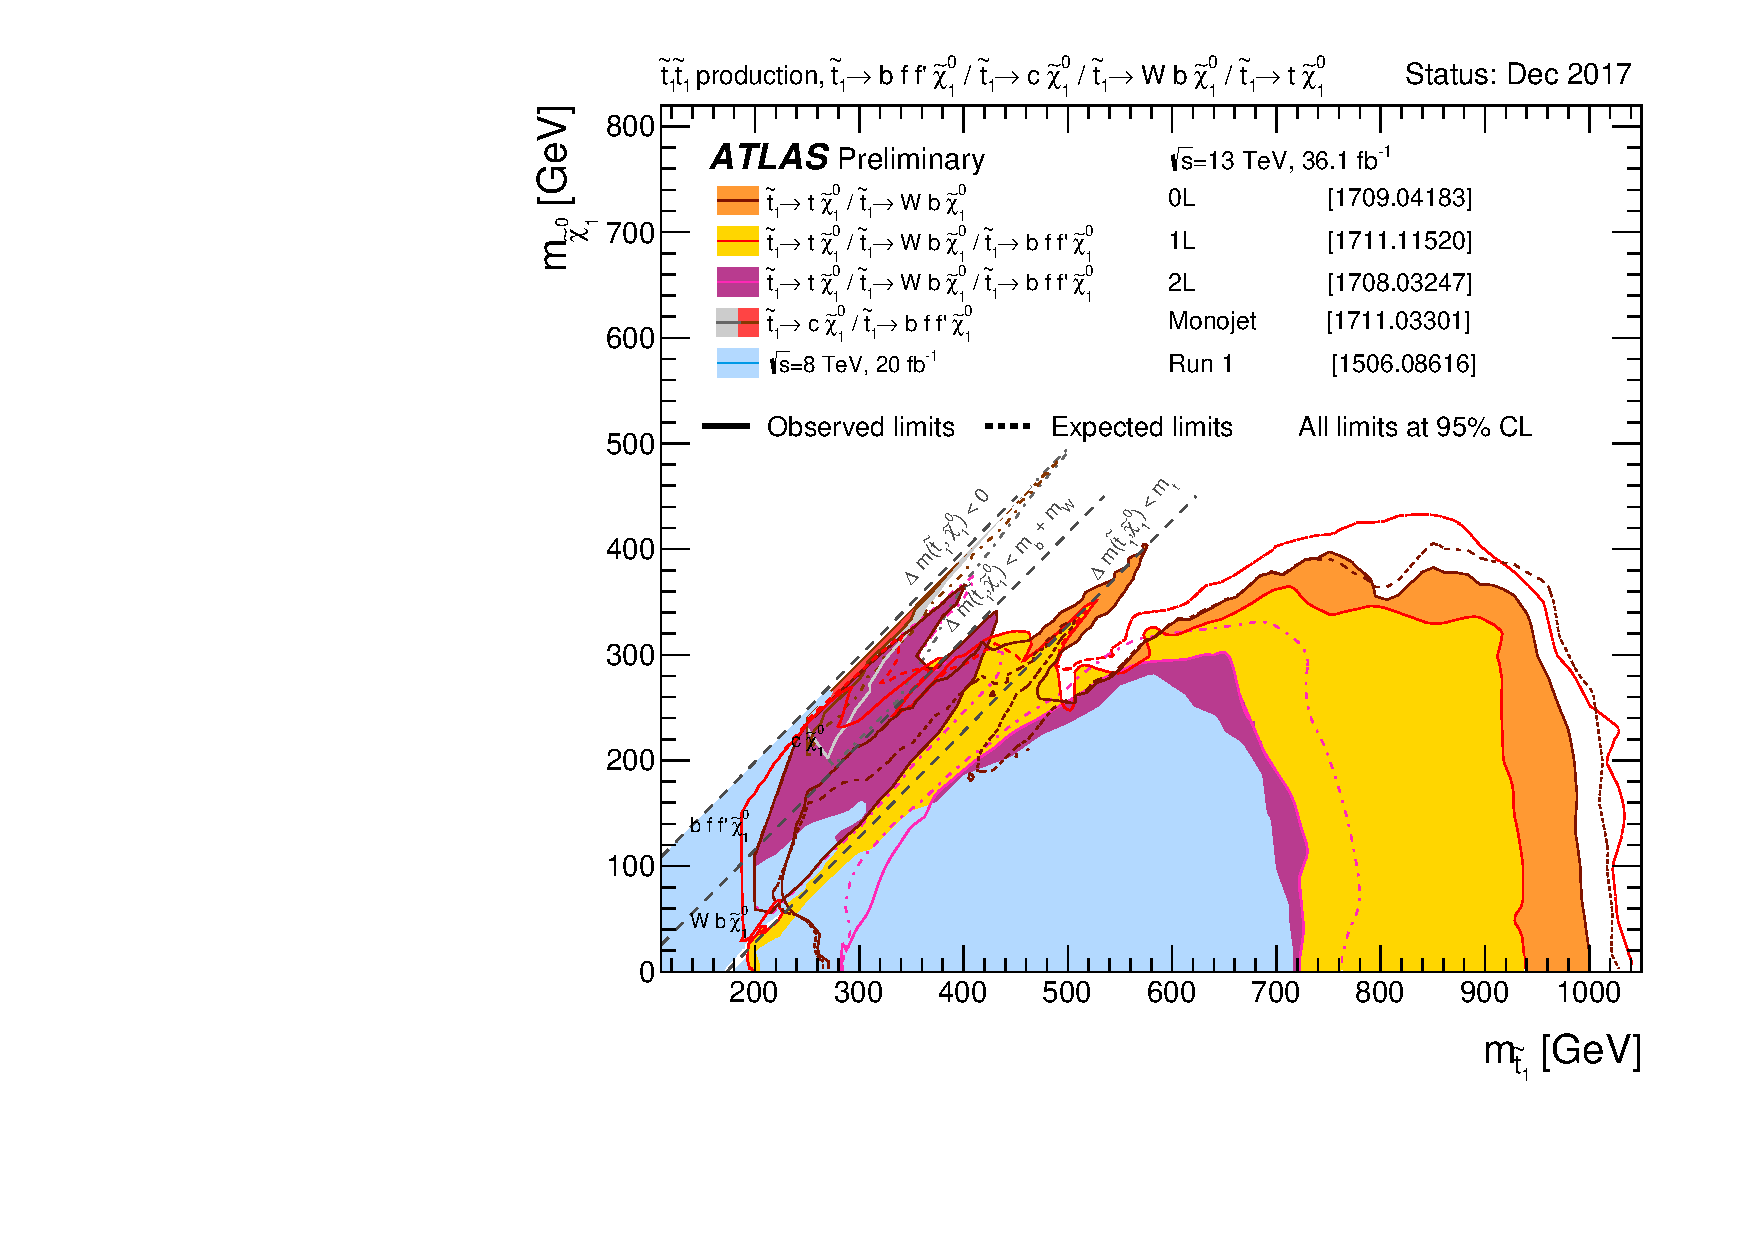
\includegraphics[width=\textwidth]{ATLAS_SUSY_Stop_tLSP}
      \end{figure}
      \vspace{-25pt}
      \begin{figure}
        \centering
        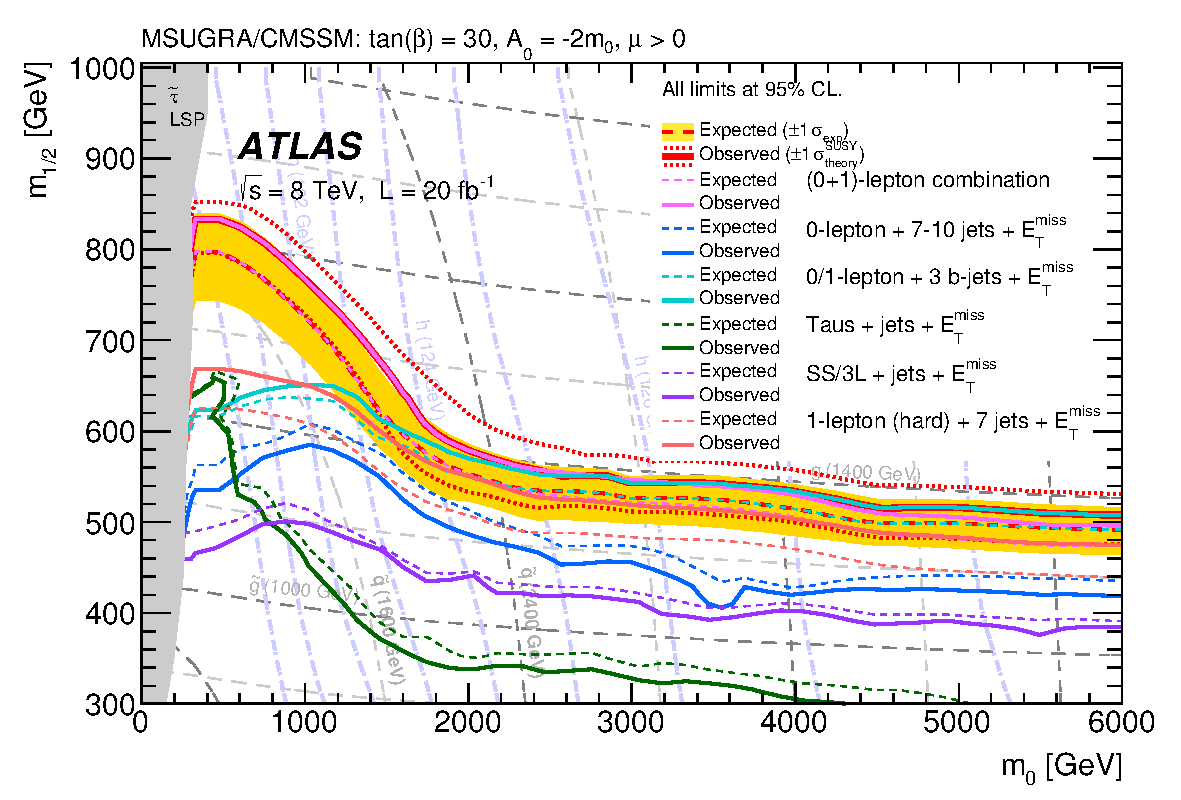
\includegraphics[width=\textwidth]{ATLAS_SUSY_MSUGRA}
      \end{figure}
      \vspace{-25pt}
      \begin{center}
        { \tiny
          [\href{http://atlas.web.cern.ch/Atlas/GROUPS/PHYSICS/CombinedSummaryPlots/SUSY/}{%
              ATLAS summary plots}]
          }
      \end{center}
    \end{column}
    \begin{column}{0.7\textwidth}
      \vspace{-20pt}
      \begin{figure}
        \centering
        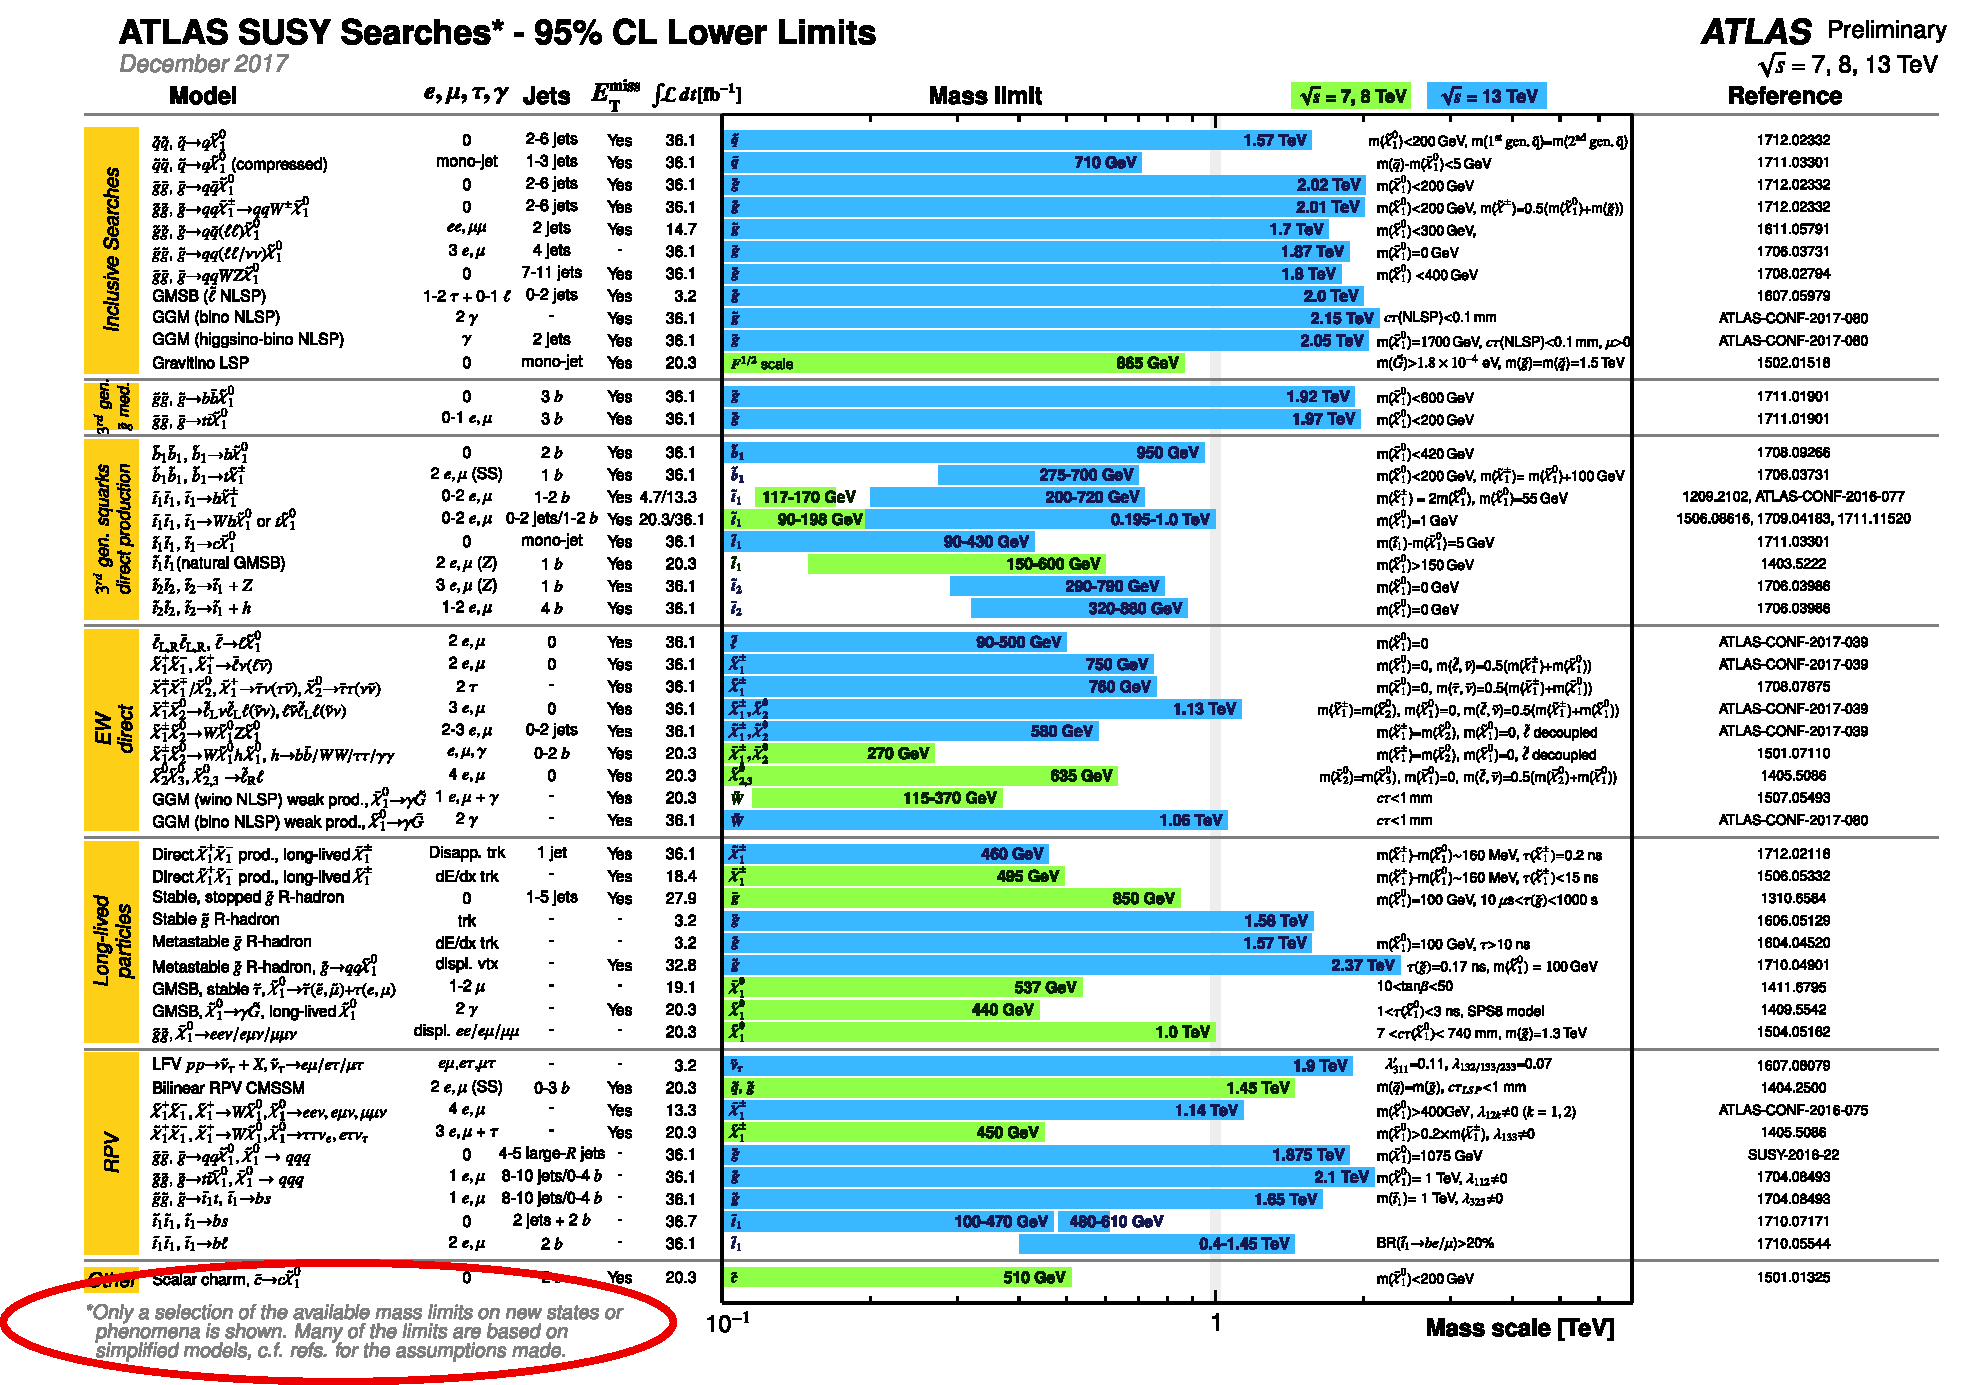
\includegraphics[width=0.8\textwidth]{ATLAS_SUSY_Summary}
      \end{figure}
      \vspace{-15pt}
      \begin{itemize}\itemsep1em
      \item Extensive collider searches $\Rightarrow$ increasingly
        stringent limits on superpartners
      \end{itemize}
    \end{column}
  \end{columns}
\end{frame}

\begin{frame}
  \frametitle{Status and Prospects of the MSSM}
  \begin{columns}[t]
    \begin{column}{0.5\textwidth}
      \vspace{-20pt}
      \begin{itemize} \itemsep1em
      \item Not just collider searches!
      \end{itemize}
      \vspace{-15pt}
      \begin{figure}
        \hspace{-10pt}
        \includegraphics[width=0.6\textwidth]{%
          cmssm_mupos1TeV_MGluMSu6_exclusions}
      \end{figure}
      \vspace{-27pt}
      \begin{center}
        { \tiny [\href{http://arxiv.org/abs/arXiv:1610.03374}{%
              arXiv:1610.03374}] }
      \end{center}
      \vspace{-15pt}
      \begin{figure}
        \hspace{-15pt}
        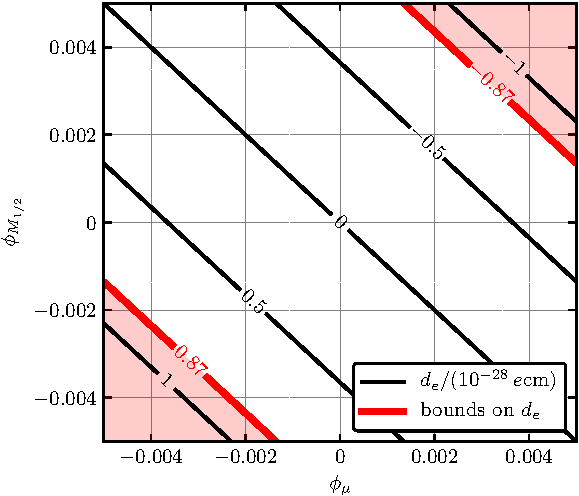
\includegraphics[width=0.5\textwidth]{contour_de_PhiMuM12}
      \end{figure}
      \vspace{-25pt}
      \begin{center}
        { \tiny [\href{http://arxiv.org/abs/arXiv:1710.03760}{%
              arXiv:1710.03760}] }
      \end{center}
    \end{column}
    \begin{column}{0.5\textwidth}
      \vspace{-20pt}
      \begin{figure}
        \hspace{-50pt}
        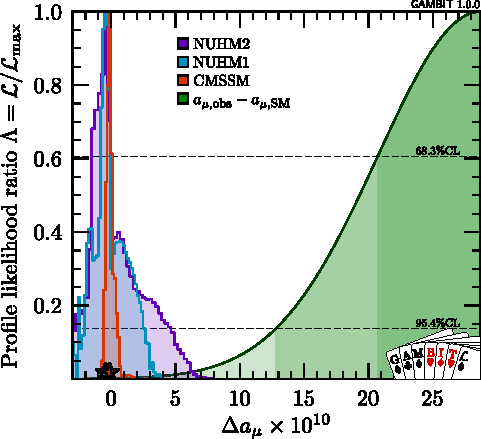
\includegraphics[width=0.5\textwidth]{gambit_gut_amu}
        \hspace{10pt}
        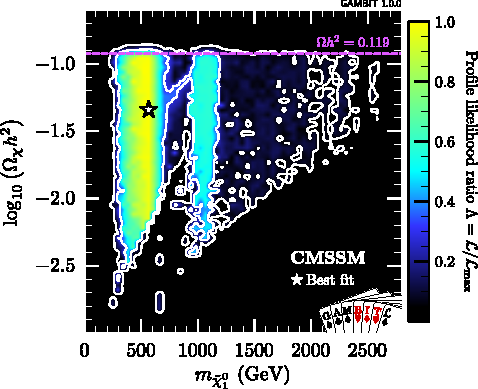
\includegraphics[width=0.55\textwidth]{gambit_gut_direct_detection}
      \end{figure}
      \vspace{-25pt}
      \begin{center}
            { \tiny [\href{http://arxiv.org/abs/1705.07935}{%
                  arXiv:1705.07935}] }
      \end{center}
      \begin{columns}[t]
        \begin{column}{0.5\textwidth}
          \vspace{-25pt}
          \begin{figure}
            \hspace{-50pt}
            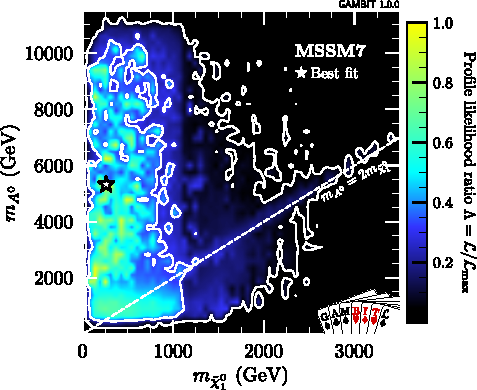
\includegraphics[width=1.1\textwidth]{gambit_mssm7_mchi_mA}
          \end{figure}
          \vspace{-25pt}
          \begin{center}
            { \tiny [\href{http://arxiv.org/abs/1705.07917}{%
                  arXiv:1705.07917}] }
          \end{center}
        \end{column}
        \begin{column}{0.5\textwidth}
          \vspace{-20pt}
          \begin{figure}
            \hspace{-15pt}
            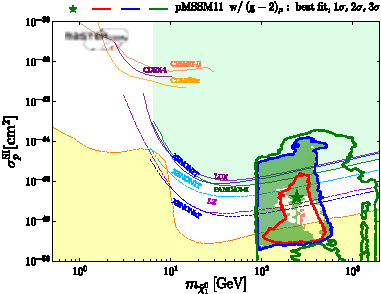
\includegraphics[width=\textwidth]{mastercode_direct_detection}
          \end{figure}
          \vspace{-20pt}
          \begin{center}
            { \tiny [\href{http://arxiv.org/abs/1710.11091}{%
                  arXiv:1710.11091}] }
          \end{center}
        \end{column}
      \end{columns}
    \end{column}
  \end{columns}
\end{frame}

% Non-minimal SUSY
\section{Non-minimal SUSY}

% - emphasise: often people equate SUSY = MSSM
% - indeed, know SM to be insufficient, so might expect MSSM also
%   to be limited
% - but no hard reason for SUSY to be minimal, can equally well
%   construct low-scale SUSY models with extended matter or
%   gauge sectors
% - these constitute non-minimal SUSY models
% - increasingly of relevance given the absence of evidence for
%   the MSSM
\begin{frame}
  \frametitle{SUSY $\not\equiv$ MSSM}
  \begin{center}
    The MSSM is \emph{a} realisation of TeV-scale SUSY, {\color{red}
      not the \emph{unique} such realisation}
  \end{center}
  \begin{itemize}\itemsep1em
  \item Ultimately, no fundamental reason for low-energy SUSY to be minimal
  \item MSSM shares some limitations of the minimal SM, e.g., $m_{\nu_i} = 0$
  \item SUSY $+$ extensions of SM at high-energies (e.g., RH neutrinos, GUTs)
    $\Rightarrow$ non-minimal SUSY models
  \item Minimal extension alone $\Rightarrow$ new puzzles/problems $\ldots$
    \begin{itemize}
      \item Best resolved in non-minimal models?
    \end{itemize}
  \end{itemize}
\end{frame}

% - examples of why you might want to extend the MSSM:
% - the little hierarchy problem: observed Higgs mass is difficult
%   to obtain in MSSM, requires heavy superpartners or large
%   mixings (pessimistic from the phenomenological point of view,
%   aesthetically somewhat against one of the common motivations
%   for SUSY, since implies large corrections to EW scale)
% - extend with new matter or gauge d.o.f. (=> extra F- or
%   D-terms in Lagrangian) raise Higgs mass
% - related: \mu problem, i.e., explain size of the \mu term
%   in the MSSM compared to soft terms
\begin{frame}
  \frametitle{The "Little Hierarchy Problem"}
   \begin{figure}
      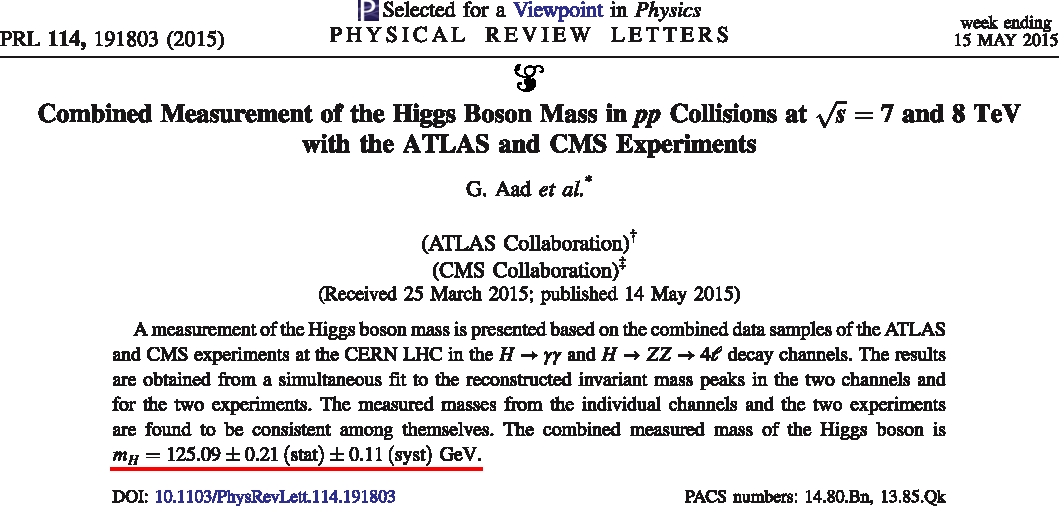
\includegraphics[width=0.75\textwidth]{higgs_mass_prl}
    \end{figure}
    \begin{center}
      MSSM tree-level prediction:
    \begin{equation*}
      m_{h_1}^2 \leq m_Z^2 \cos^2 2\beta \lesssim (91 \text{ GeV})^2
   \end{equation*}
 \end{center}
\end{frame}

\begin{frame}
  \frametitle{The "Little Hierarchy Problem"}
  \begin{itemize}\itemsep1em
    \item $m_{h_1} \approx 125$ GeV $\Rightarrow$ large higher order
      corrections
      \begin{equation*}
        m_{h_1}^2 \approx m_Z^2 \cos^2 2\beta \left ( 1 - \frac{3}{8\pi^2}
          \frac{m_t^2}{v^2} \ln \frac{m_{\tilde{t}_1} m_{\tilde{t}_2}}{M_t^2}
          \right ) {+ \color{blue} \frac{3}{4\pi^2} \frac{m_t^4}{v^2} \ln
          \frac{m_{\tilde{t}_1} m_{\tilde{t}_2}}{M_t^2}} + \ldots
      \end{equation*}
    \item $\Rightarrow$ also large corrections to prediction for $m_Z$
      at SUSY scale $M_S$:
      \begin{equation*}
        \frac{m_Z^2}{2} = -\mu^2 + \frac{\overbrace{{\color{red} m_{H_d}^2} -
          {\color{red} m_{H_u}^2}}^{\text{RGE effects}} \tan^2\beta}
          {\tan^2\beta - 1} {\color{red} +  \delta_{1-\textrm{loop}}} ,
      \end{equation*}
      \begin{equation*}
          {\color{red}
          \delta_{1-\textrm{loop}} = \frac{3}{8\pi^2} \frac{m_t^2}{v^2
            \cos 2\beta} \left [ m_{\tilde{t}_1}^2 \left ( \ln
            \frac{m_{\tilde{t}_1}^2}{M_S^2} - 1 \right ) + m_{\tilde{t}_2}^2
            \left ( \ln \frac{m_{\tilde{t}_2}^2}{M_S^2} - 1 \right ) \right ]
            + \ldots }
      \end{equation*}
    \item $\Rightarrow$ naturalness problem?
    \item \alert{$\mu$-problem}: $m_Z^2/2 = -\mu^2 + \ldots \Rightarrow \mu
      \sim$ soft parameters?
  \end{itemize}
\end{frame}

% - mention shortcoming: give up minimality, what guides model-building?
% - obviously, non-minimal model must still reproduce SM results
% - otherwise extreme freedom: new matter fields, new gauge symmetries
% - guiding principle? E.g., some models can be seen to emerge from
%   UV complete theories (GUTs, strings, ...)
% - later can then mention Bayesian naturalness work as means of
%   discriminating between different models
\begin{frame}
  \frametitle{Going Beyond the MSSM}
\end{frame}

% simple example of non-minimal model doing this: the NMSSM
% - introduce NMSSM, simplest such extension where add a single
%   SM singlet superfield
% - positive features: larger Higgs mass, explains \mu problem
%   dynamically, improved prospects for e.g. baryogenesis
\begin{frame}
  \frametitle{Example: The NMSSM}
\end{frame}

% - no (concrete) evidence for MSSM or NMSSM, why would we consider then
%   a more complicated model?
% - can frame in context of Bayesian statistics, given the
%   observed limits can assess (given some set of priors)
%   plausibility of one versus the other
% - incorporates traditional, ad hoc fine tuning arguments
%   automatically
\begin{frame}
  \frametitle{Ockham's Razor}
  % Numquam ponenda est pluralitas sine necessitate
\end{frame}

% further reasons for extending the MSSM
% - improved gauge unification in the MSSM
%   => embed in a GUT model at high-energies?
% - motivates considerations of SUSY GUTs, e.g., SUSY SO(10),
%   E_6
% - emerge naturally in the context of superstring theory,
%   i.e., candidate theories of gravity, where breakdown of
%   SUSY in hidden sector is communicated to visible sector by
%   gravitational strength interactions (remind earlier discussion
%   of Planck mediated breaking)
% - rich phenomenology if exotic states survive to low energies
\begin{frame}
  \frametitle{Going Further}
\end{frame}

% example: the E6SSM and its variants
% - summarise some of the interesting features: general model
%   construction goes through as usual, matter embedded in complete
%   E6 reps => exotic coloured states
% - resolve \mu problem and avoid issues that come with scale-free
%   NMSSM, raise Higgs mass even further
% - briefly discuss some model building complications (e.g. Z2
%   symmetries), can resolve with E6 variants but do not go into
%   extensive detail
\begin{frame}
  \frametitle{$U(1)$ Extensions of the MSSM}
    \begin{equation*}
      SU(3)_C \times SU(2)_L \times U(1)_Y \to
      SU(3)_C \times SU(2)_L \times U(1)_Y \times U(1)^\prime
    \end{equation*}
    \vspace{-15pt}
  \begin{columns}[t]
    \begin{column}{0.45\textwidth}
      \begin{itemize} \itemsep1em
        \item Well-motivated extensions of MSSM, NMSSM
        \item $W_{\text{USSM}} \supset \lambda \hat{S} H_d
          \cdot H_u$, $Q^\prime_{\hat{S}} \neq 0$ $\Rightarrow$
          $\langle S \rangle = s / \sqrt{2}$ also breaks $U(1)^\prime$,
          generating {\color{blue} massive $Z^\prime$}
        \item Consistent model requires anomaly cancellation
          \begin{itemize}
            \item either family non-universal $U(1)^\prime$ charges
              or {\color{blue} extra matter}
          \end{itemize}
        \item Additional states $\Rightarrow$ exciting phenomenology
      \end{itemize}
    \end{column}
    \begin{column}{0.6\textwidth}
      \vspace{-10pt}
      \begin{figure}
        \centering
        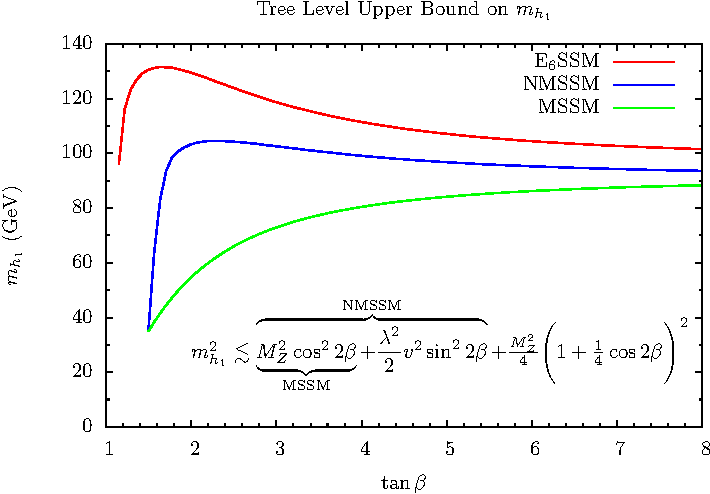
\includegraphics[width=\textwidth]{treelevel_higgs_upperbound_plot}
      \end{figure}
    \end{column}
  \end{columns}
\end{frame}

\begin{frame}
  \frametitle{$E_6$ Inspired Models}
  \begin{itemize} \itemsep1em
     \item Lead to $U(1)$ extended models at low-energies:
      \begin{align*}
        E_6&\longrightarrow SO(10)\times U(1)_\psi \\
        &\longrightarrow SU(5)\times U(1)_\psi\times U(1)_\chi\\
        &\longrightarrow SU(3)_C\times SU(2)_L\times U(1)_Y\times
        U(1)_\psi\times U(1)_\chi\\
        &\longrightarrow SU(3)_C\times SU(2)_L\times U(1)_Y\times
        U(1)^\prime
      \end{align*}
    \item Resulting charges $Q' = Q_\chi \cos \theta_{E_6}
      + Q_\psi \sin \theta_{E_6}$, e.g., class of models
      \begin{table}[h]
        \begin{tabular}{cl}
          $U(1)_N$: & $Q_N = Q(\theta_{E_6} = \arctan\sqrt{15})$
            ($\equiv$ E$_6$SSM) \\
          $U(1)_\psi$: & $Q_\psi = Q(\theta_{E_6} = \pi / 2)$\\
          $U(1)_\eta$: & $Q_\eta = -Q(\theta_{E_6} = \pi -
            \arctan\sqrt{5/3})$\\
          $U(1)_I$: & $Q_I = -Q(\theta_{E_6} = \arctan\sqrt{3/5})$
        \end{tabular}
      \end{table}
    \item Matter content fills complete $\mathbf{27}$ representations
      ({\color{blue} ensures anomaly cancellation})
      \begin{itemize}
        \item $\Rightarrow$ additional exotic states
      \end{itemize}
  \end{itemize}
\end{frame}

\begin{frame}
  \frametitle{The E$_6$SSM}
    \begin{columns}[t]
      \begin{column}{0.5\textwidth}
        \begin{itemize} \itemsep0.2em
        \item $\tan\theta_{E_6} = \sqrt{15}$ $\Rightarrow$ $U(1)_N$
          under which right-handed neutrinos are uncharged
          \begin{itemize}
            \item allows {\color{blue} $\nu$ masses via see-saw} and
              {\color{blue} successful baryogenesis} [1]
          \end{itemize}
        \item Extra $L_4$, $\hat{\overline{L}}_4$ from incomplete
          $\mathbf{27}^\prime$, $\mathbf{\overline{27}}^\prime$ for gauge
          unification
        \item Low-energy matter content from $\mathbf{27}$-plet:
          \begin{align*}
            &(Q_i, \, \hat{u}^c_i, \, \hat{d}^c_i, \, L_i, \,
            e^c_i) + (\hat{D}_i, \, \hat{\overline{D}}_i)\\
            &\quad {} + (\hat{S}_{i}) + (H^u_i) + (H^d_i)
          \end{align*}
        \item Higgs doublets $H^d_3$, $H^u_3$ and one singlet
          $\hat{S}_3$ get VEVs ($\Rightarrow$ EWSB and break $U(1)_N$)
          \vfill
        \end{itemize}
      \end{column}
      \begin{column}{0.5\textwidth}
        \vspace{-40pt}
        \begin{table}[h]
          \centering
          \begin{tabular}{ccccc}
            \toprule
            & $SU(3)_C$ & $SU(2)_L$ & $\sqrt{\frac{5}{3}} Q_i^Y$
            & $\sqrt{40} Q_i^N$ \\
            \midrule
            $Q_i$ & $\mathbf{3}$ & $\mathbf{2}$ & $\frac{1}{6}$ & $1$ \\
            $\hat{u}_i^c$ & $\mathbf{\overline{3}}$ & $\mathbf{1}$
            & $-\frac{2}{3}$ & $1$ \\
            $\hat{d}_i^c$ & $\mathbf{\overline{3}}$ & $\mathbf{1}$
            & $\frac{1}{3}$ & $2$ \\
            $L_i$ & $\mathbf{1}$ & $\mathbf{2}$ & $-\frac{1}{2}$ & $2$ \\
            $e_i^c$ & $\mathbf{1}$ & $\mathbf{1}$ & $1$ & $1$ \\
            $\hat{S}_i$ & $\mathbf{1}$ & $\mathbf{1}$ & $0$ & $5$ \\
            $H_i^u$ & $\mathbf{1}$ & $\mathbf{2}$ & $\frac{1}{2}$
            & $-2$ \\
            $H_i^d$ & $\mathbf{1}$ & $\mathbf{2}$ & $-\frac{1}{2}$
            & $-3$ \\
            $\hat{D}$ & $\mathbf{3}$ & $\mathbf{1}$ & $-\frac{1}{3}$ & $-2$ \\
            $\hat{\overline{D}}$ & $\mathbf{\overline{3}}$ &  $\mathbf{1}$
            & $\frac{1}{3}$ & $-3$ \\
            $L_4$ & $\mathbf{1}$ & $\mathbf{2}$ & $-\frac{1}{2}$ & $2$ \\
            $\hat{\overline{L}}_4$ & $\mathbf{1}$ & $\mathbf{\overline{2}}$
            & $\frac{1}{2}$ & $-2$ \\
            \bottomrule
          \end{tabular}
        \end{table}
      \end{column}
    \end{columns}
    \vspace{-4pt}
    \begin{align*}
      \Aboxed{W_{\text{E}_6\text{SSM}} \approx y_{\tau} L_3 \cdot
        H^d_3 e^c_3 + y_b Q_3 \cdot H^d_3 \hat{d}_3^c
        + y_t H^u_3 \cdot Q_3 \hat{u}_3^c + \lambda_i \hat{S}_3
        H_i^d \cdot H_i^u  + \kappa_i \hat{S}_3 \hat{D}_i
        \hat{\overline{D}}_i + \mu_L L_4 \cdot \hat{\overline{L}}_4}
    \end{align*}
        {\tiny [1] S.~F.~King, S.~Moretti, and R.~Nevzorov,
          \href{http://dx.doi.org/10.1103/PhysRevD.73.035009}{Phys.~Rev.~D
            \textbf{73}, 035009 (2006)}
          (\href{http://arxiv.org/abs/hep-ph/0510419}{hep-ph/0510419})}
\end{frame}

\begin{frame}
  \frametitle{Experimental Signatures of the E$_6$SSM}
\end{frame}

\begin{frame}
  \frametitle{Limitations of Simple $E_6$ Models}
\end{frame}

\section{Summary}

\begin{frame}
  \frametitle{Summary}

  \begin{center}
    \large Thank you for listening!
  \end{center}

\end{frame}

\appendix

\begin{frame}
  \begin{center}
    {
      \Large
      Additional Slides
    }
  \end{center}
\end{frame}

% construction of Minkowski space as coset space of Poincare
% group factored by Lorentz group, analogy for superspace?

\begin{frame}
  \frametitle{Differentiation for Grassmann Variables}
\end{frame}

\begin{frame}
  \frametitle{Component Field Form of SUSY Lagrangian}
\end{frame}

\end{document}
